\documentclass[anon,12pt]{colt2024} % Anonymized submission
%\documentclass[final,12pt]{colt2024} % Include author names
%\usepackage{graphicx}
% The following packages will be automatically loaded:
% amsmath, amssymb, natbib, graphicx, url, algorithm2e

\title[Reconstruction of Random Hypergraphs]{Thresholds for Reconstruction of Random Hypergraphs \\ From Graph Projections}
\usepackage{times}
% Use \Name{Author Name} to specify the name.
% If the surname contains spaces, enclose the surname
% in braces, e.g. \Name{John {Smith Jones}} similarly
% if the name has a "von" part, e.g \Name{Jane {de Winter}}.
% If the first letter in the forenames is a diacritic
% enclose the diacritic in braces, e.g. \Name{{\'E}louise Smith}

% Two authors with the same address
% \coltauthor{\Name{Author Name1} \Email{abc@sample.com}\and
%  \Name{Author Name2} \Email{xyz@sample.com}\\
%  \addr Address}

% Three or more authors with the same address:
% \coltauthor{\Name{Author Name1} \Email{an1@sample.com}\\
%  \Name{Author Name2} \Email{an2@sample.com}\\
%  \Name{Author Name3} \Email{an3@sample.com}\\
%  \addr Address}

% Authors with different addresses:
\coltauthor{%
 \Name{Guy Bresler} \Email{guy@mit.edu}\\
 \addr 32-D672, 32 Vassar St., Cambridge, MA 02139%
 \AND
 \Name{Chenghao Guo} \Email{chenghao@mit.edu}\\
 \addr 32-D678, 32 Vassar St., Cambridge, MA 02139%
 \AND
 \Name{Yury Polyanskiy} \Email{yp@mit.edu}\\
 \addr 32-D678, 32 Vassar St., Cambridge, MA 02139%
}


%
\setlength\unitlength{1mm}
\newcommand{\twodots}{\mathinner {\ldotp \ldotp}}
% bb font symbols
\newcommand{\Rho}{\mathrm{P}}
\newcommand{\Tau}{\mathrm{T}}

\newfont{\bbb}{msbm10 scaled 700}
\newcommand{\CCC}{\mbox{\bbb C}}

\newfont{\bb}{msbm10 scaled 1100}
\newcommand{\CC}{\mbox{\bb C}}
\newcommand{\PP}{\mbox{\bb P}}
\newcommand{\RR}{\mbox{\bb R}}
\newcommand{\QQ}{\mbox{\bb Q}}
\newcommand{\ZZ}{\mbox{\bb Z}}
\newcommand{\FF}{\mbox{\bb F}}
\newcommand{\GG}{\mbox{\bb G}}
\newcommand{\EE}{\mbox{\bb E}}
\newcommand{\NN}{\mbox{\bb N}}
\newcommand{\KK}{\mbox{\bb K}}
\newcommand{\HH}{\mbox{\bb H}}
\newcommand{\SSS}{\mbox{\bb S}}
\newcommand{\UU}{\mbox{\bb U}}
\newcommand{\VV}{\mbox{\bb V}}


\newcommand{\yy}{\mathbbm{y}}
\newcommand{\xx}{\mathbbm{x}}
\newcommand{\zz}{\mathbbm{z}}
\newcommand{\sss}{\mathbbm{s}}
\newcommand{\rr}{\mathbbm{r}}
\newcommand{\pp}{\mathbbm{p}}
\newcommand{\qq}{\mathbbm{q}}
\newcommand{\ww}{\mathbbm{w}}
\newcommand{\hh}{\mathbbm{h}}
\newcommand{\vvv}{\mathbbm{v}}

% Vectors

\newcommand{\av}{{\bf a}}
\newcommand{\bv}{{\bf b}}
\newcommand{\cv}{{\bf c}}
\newcommand{\dv}{{\bf d}}
\newcommand{\ev}{{\bf e}}
\newcommand{\fv}{{\bf f}}
\newcommand{\gv}{{\bf g}}
\newcommand{\hv}{{\bf h}}
\newcommand{\iv}{{\bf i}}
\newcommand{\jv}{{\bf j}}
\newcommand{\kv}{{\bf k}}
\newcommand{\lv}{{\bf l}}
\newcommand{\mv}{{\bf m}}
\newcommand{\nv}{{\bf n}}
\newcommand{\ov}{{\bf o}}
\newcommand{\pv}{{\bf p}}
\newcommand{\qv}{{\bf q}}
\newcommand{\rv}{{\bf r}}
\newcommand{\sv}{{\bf s}}
\newcommand{\tv}{{\bf t}}
\newcommand{\uv}{{\bf u}}
\newcommand{\wv}{{\bf w}}
\newcommand{\vv}{{\bf v}}
\newcommand{\xv}{{\bf x}}
\newcommand{\yv}{{\bf y}}
\newcommand{\zv}{{\bf z}}
\newcommand{\zerov}{{\bf 0}}
\newcommand{\onev}{{\bf 1}}

% Matrices

\newcommand{\Am}{{\bf A}}
\newcommand{\Bm}{{\bf B}}
\newcommand{\Cm}{{\bf C}}
\newcommand{\Dm}{{\bf D}}
\newcommand{\Em}{{\bf E}}
\newcommand{\Fm}{{\bf F}}
\newcommand{\Gm}{{\bf G}}
\newcommand{\Hm}{{\bf H}}
\newcommand{\Id}{{\bf I}}
\newcommand{\Jm}{{\bf J}}
\newcommand{\Km}{{\bf K}}
\newcommand{\Lm}{{\bf L}}
\newcommand{\Mm}{{\bf M}}
\newcommand{\Nm}{{\bf N}}
\newcommand{\Om}{{\bf O}}
\newcommand{\Pm}{{\bf P}}
\newcommand{\Qm}{{\bf Q}}
\newcommand{\Rm}{{\bf R}}
\newcommand{\Sm}{{\bf S}}
\newcommand{\Tm}{{\bf T}}
\newcommand{\Um}{{\bf U}}
\newcommand{\Wm}{{\bf W}}
\newcommand{\Vm}{{\bf V}}
\newcommand{\Xm}{{\bf X}}
\newcommand{\Ym}{{\bf Y}}
\newcommand{\Zm}{{\bf Z}}

% Calligraphic

\newcommand{\Ac}{{\cal A}}
\newcommand{\Bc}{{\cal B}}
\newcommand{\Cc}{{\cal C}}
\newcommand{\Dc}{{\cal D}}
\newcommand{\Ec}{{\cal E}}
\newcommand{\Fc}{{\cal F}}
\newcommand{\Gc}{{\cal G}}
\newcommand{\Hc}{{\cal H}}
\newcommand{\Ic}{{\cal I}}
\newcommand{\Jc}{{\cal J}}
\newcommand{\Kc}{{\cal K}}
\newcommand{\Lc}{{\cal L}}
\newcommand{\Mc}{{\cal M}}
\newcommand{\Nc}{{\cal N}}
\newcommand{\nc}{{\cal n}}
\newcommand{\Oc}{{\cal O}}
\newcommand{\Pc}{{\cal P}}
\newcommand{\Qc}{{\cal Q}}
\newcommand{\Rc}{{\cal R}}
\newcommand{\Sc}{{\cal S}}
\newcommand{\Tc}{{\cal T}}
\newcommand{\Uc}{{\cal U}}
\newcommand{\Wc}{{\cal W}}
\newcommand{\Vc}{{\cal V}}
\newcommand{\Xc}{{\cal X}}
\newcommand{\Yc}{{\cal Y}}
\newcommand{\Zc}{{\cal Z}}

% Bold greek letters

\newcommand{\alphav}{\hbox{\boldmath$\alpha$}}
\newcommand{\betav}{\hbox{\boldmath$\beta$}}
\newcommand{\gammav}{\hbox{\boldmath$\gamma$}}
\newcommand{\deltav}{\hbox{\boldmath$\delta$}}
\newcommand{\etav}{\hbox{\boldmath$\eta$}}
\newcommand{\lambdav}{\hbox{\boldmath$\lambda$}}
\newcommand{\epsilonv}{\hbox{\boldmath$\epsilon$}}
\newcommand{\nuv}{\hbox{\boldmath$\nu$}}
\newcommand{\muv}{\hbox{\boldmath$\mu$}}
\newcommand{\zetav}{\hbox{\boldmath$\zeta$}}
\newcommand{\phiv}{\hbox{\boldmath$\phi$}}
\newcommand{\psiv}{\hbox{\boldmath$\psi$}}
\newcommand{\thetav}{\hbox{\boldmath$\theta$}}
\newcommand{\tauv}{\hbox{\boldmath$\tau$}}
\newcommand{\omegav}{\hbox{\boldmath$\omega$}}
\newcommand{\xiv}{\hbox{\boldmath$\xi$}}
\newcommand{\sigmav}{\hbox{\boldmath$\sigma$}}
\newcommand{\piv}{\hbox{\boldmath$\pi$}}
\newcommand{\rhov}{\hbox{\boldmath$\rho$}}
\newcommand{\upsilonv}{\hbox{\boldmath$\upsilon$}}

\newcommand{\Gammam}{\hbox{\boldmath$\Gamma$}}
\newcommand{\Lambdam}{\hbox{\boldmath$\Lambda$}}
\newcommand{\Deltam}{\hbox{\boldmath$\Delta$}}
\newcommand{\Sigmam}{\hbox{\boldmath$\Sigma$}}
\newcommand{\Phim}{\hbox{\boldmath$\Phi$}}
\newcommand{\Pim}{\hbox{\boldmath$\Pi$}}
\newcommand{\Psim}{\hbox{\boldmath$\Psi$}}
\newcommand{\Thetam}{\hbox{\boldmath$\Theta$}}
\newcommand{\Omegam}{\hbox{\boldmath$\Omega$}}
\newcommand{\Xim}{\hbox{\boldmath$\Xi$}}


% Sans Serif small case

\newcommand{\Gsf}{{\sf G}}

\newcommand{\asf}{{\sf a}}
\newcommand{\bsf}{{\sf b}}
\newcommand{\csf}{{\sf c}}
\newcommand{\dsf}{{\sf d}}
\newcommand{\esf}{{\sf e}}
\newcommand{\fsf}{{\sf f}}
\newcommand{\gsf}{{\sf g}}
\newcommand{\hsf}{{\sf h}}
\newcommand{\isf}{{\sf i}}
\newcommand{\jsf}{{\sf j}}
\newcommand{\ksf}{{\sf k}}
\newcommand{\lsf}{{\sf l}}
\newcommand{\msf}{{\sf m}}
\newcommand{\nsf}{{\sf n}}
\newcommand{\osf}{{\sf o}}
\newcommand{\psf}{{\sf p}}
\newcommand{\qsf}{{\sf q}}
\newcommand{\rsf}{{\sf r}}
\newcommand{\ssf}{{\sf s}}
\newcommand{\tsf}{{\sf t}}
\newcommand{\usf}{{\sf u}}
\newcommand{\wsf}{{\sf w}}
\newcommand{\vsf}{{\sf v}}
\newcommand{\xsf}{{\sf x}}
\newcommand{\ysf}{{\sf y}}
\newcommand{\zsf}{{\sf z}}


% mixed symbols

\newcommand{\sinc}{{\hbox{sinc}}}
\newcommand{\diag}{{\hbox{diag}}}
\renewcommand{\det}{{\hbox{det}}}
\newcommand{\trace}{{\hbox{tr}}}
\newcommand{\sign}{{\hbox{sign}}}
\renewcommand{\arg}{{\hbox{arg}}}
\newcommand{\var}{{\hbox{var}}}
\newcommand{\cov}{{\hbox{cov}}}
\newcommand{\Ei}{{\rm E}_{\rm i}}
\renewcommand{\Re}{{\rm Re}}
\renewcommand{\Im}{{\rm Im}}
\newcommand{\eqdef}{\stackrel{\Delta}{=}}
\newcommand{\defines}{{\,\,\stackrel{\scriptscriptstyle \bigtriangleup}{=}\,\,}}
\newcommand{\<}{\left\langle}
\renewcommand{\>}{\right\rangle}
\newcommand{\herm}{{\sf H}}
\newcommand{\trasp}{{\sf T}}
\newcommand{\transp}{{\sf T}}
\renewcommand{\vec}{{\rm vec}}
\newcommand{\Psf}{{\sf P}}
\newcommand{\SINR}{{\sf SINR}}
\newcommand{\SNR}{{\sf SNR}}
\newcommand{\MMSE}{{\sf MMSE}}
\newcommand{\REF}{{\RED [REF]}}

% Markov chain
\usepackage{stmaryrd} % for \mkv 
\newcommand{\mkv}{-\!\!\!\!\minuso\!\!\!\!-}

% Colors

\newcommand{\RED}{\color[rgb]{1.00,0.10,0.10}}
\newcommand{\BLUE}{\color[rgb]{0,0,0.90}}
\newcommand{\GREEN}{\color[rgb]{0,0.80,0.20}}

%%%%%%%%%%%%%%%%%%%%%%%%%%%%%%%%%%%%%%%%%%
\usepackage{hyperref}
\hypersetup{
    bookmarks=true,         % show bookmarks bar?
    unicode=false,          % non-Latin characters in AcrobatÕs bookmarks
    pdftoolbar=true,        % show AcrobatÕs toolbar?
    pdfmenubar=true,        % show AcrobatÕs menu?
    pdffitwindow=false,     % window fit to page when opened
    pdfstartview={FitH},    % fits the width of the page to the window
%    pdftitle={My title},    % title
%    pdfauthor={Author},     % author
%    pdfsubject={Subject},   % subject of the document
%    pdfcreator={Creator},   % creator of the document
%    pdfproducer={Producer}, % producer of the document
%    pdfkeywords={keyword1} {key2} {key3}, % list of keywords
    pdfnewwindow=true,      % links in new window
    colorlinks=true,       % false: boxed links; true: colored links
    linkcolor=red,          % color of internal links (change box color with linkbordercolor)
    citecolor=green,        % color of links to bibliography
    filecolor=blue,      % color of file links
    urlcolor=blue           % color of external links
}
%%%%%%%%%%%%%%%%%%%%%%%%%%%%%%%%%%%%%%%%%%%



\begin{document}

\maketitle
\begin{abstract}
The \emph{graph projection} of a hypergraph is a simple graph with the same vertex set and with an edge between each pair of vertices that appear in a hyperedge.  
We consider the problem of reconstructing a random $d$-uniform hypergraph from its projection. Feasibility of this task depends on $d$ and the density of hyperedges in the random hypergraph. For $d=3$ we precisely determine the threshold, while for $d\geq 4$ we give bounds. All of our feasibility results are obtained by exhibiting an efficient algorithm for reconstructing the original hypergraph, while infeasibility is information-theoretic. 

Our results also apply to mildly inhomogeneous random hypergrahps, including hypergraph stochastic block models. A consequence of our results is that claims from the 2023 COLT paper \cite{gaudio2023community} are disproved. 
\end{abstract}

\begin{keywords}%
Hypergraph, Random Graph, Exact Recovery%
\end{keywords}

\section{Introduction}

Large language models (LLMs) have achieved remarkable success in automated math problem solving, particularly through code-generation capabilities integrated with proof assistants~\citep{lean,isabelle,POT,autoformalization,MATH}. Although LLMs excel at generating solution steps and correct answers in algebra and calculus~\citep{math_solving}, their unimodal nature limits performance in plane geometry, where solution depends on both diagram and text~\citep{math_solving}. 

Specialized vision-language models (VLMs) have accordingly been developed for plane geometry problem solving (PGPS)~\citep{geoqa,unigeo,intergps,pgps,GOLD,LANS,geox}. Yet, it remains unclear whether these models genuinely leverage diagrams or rely almost exclusively on textual features. This ambiguity arises because existing PGPS datasets typically embed sufficient geometric details within problem statements, potentially making the vision encoder unnecessary~\citep{GOLD}. \cref{fig:pgps_examples} illustrates example questions from GeoQA and PGPS9K, where solutions can be derived without referencing the diagrams.

\begin{figure}
    \centering
    \begin{subfigure}[t]{.49\linewidth}
        \centering
        \includegraphics[width=\linewidth]{latex/figures/images/geoqa_example.pdf}
        \caption{GeoQA}
        \label{fig:geoqa_example}
    \end{subfigure}
    \begin{subfigure}[t]{.48\linewidth}
        \centering
        \includegraphics[width=\linewidth]{latex/figures/images/pgps_example.pdf}
        \caption{PGPS9K}
        \label{fig:pgps9k_example}
    \end{subfigure}
    \caption{
    Examples of diagram-caption pairs and their solution steps written in formal languages from GeoQA and PGPS9k datasets. In the problem description, the visual geometric premises and numerical variables are highlighted in green and red, respectively. A significant difference in the style of the diagram and formal language can be observable. %, along with the differences in formal languages supported by the corresponding datasets.
    \label{fig:pgps_examples}
    }
\end{figure}



We propose a new benchmark created via a synthetic data engine, which systematically evaluates the ability of VLM vision encoders to recognize geometric premises. Our empirical findings reveal that previously suggested self-supervised learning (SSL) approaches, e.g., vector quantized variataional auto-encoder (VQ-VAE)~\citep{unimath} and masked auto-encoder (MAE)~\citep{scagps,geox}, and widely adopted encoders, e.g., OpenCLIP~\citep{clip} and DinoV2~\citep{dinov2}, struggle to detect geometric features such as perpendicularity and degrees. 

To this end, we propose \geoclip{}, a model pre-trained on a large corpus of synthetic diagram–caption pairs. By varying diagram styles (e.g., color, font size, resolution, line width), \geoclip{} learns robust geometric representations and outperforms prior SSL-based methods on our benchmark. Building on \geoclip{}, we introduce a few-shot domain adaptation technique that efficiently transfers the recognition ability to real-world diagrams. We further combine this domain-adapted GeoCLIP with an LLM, forming a domain-agnostic VLM for solving PGPS tasks in MathVerse~\citep{mathverse}. 
%To accommodate diverse diagram styles and solution formats, we unify the solution program languages across multiple PGPS datasets, ensuring comprehensive evaluation. 

In our experiments on MathVerse~\citep{mathverse}, which encompasses diverse plane geometry tasks and diagram styles, our VLM with a domain-adapted \geoclip{} consistently outperforms both task-specific PGPS models and generalist VLMs. 
% In particular, it achieves higher accuracy on tasks requiring geometric-feature recognition, even when critical numerical measurements are moved from text to diagrams. 
Ablation studies confirm the effectiveness of our domain adaptation strategy, showing improvements in optical character recognition (OCR)-based tasks and robust diagram embeddings across different styles. 
% By unifying the solution program languages of existing datasets and incorporating OCR capability, we enable a single VLM, named \geovlm{}, to handle a broad class of plane geometry problems.

% Contributions
We summarize the contributions as follows:
We propose a novel benchmark for systematically assessing how well vision encoders recognize geometric premises in plane geometry diagrams~(\cref{sec:visual_feature}); We introduce \geoclip{}, a vision encoder capable of accurately detecting visual geometric premises~(\cref{sec:geoclip}), and a few-shot domain adaptation technique that efficiently transfers this capability across different diagram styles (\cref{sec:domain_adaptation});
We show that our VLM, incorporating domain-adapted GeoCLIP, surpasses existing specialized PGPS VLMs and generalist VLMs on the MathVerse benchmark~(\cref{sec:experiments}) and effectively interprets diverse diagram styles~(\cref{sec:abl}).

\iffalse
\begin{itemize}
    \item We propose a novel benchmark for systematically assessing how well vision encoders recognize geometric premises, e.g., perpendicularity and angle measures, in plane geometry diagrams.
	\item We introduce \geoclip{}, a vision encoder capable of accurately detecting visual geometric premises, and a few-shot domain adaptation technique that efficiently transfers this capability across different diagram styles.
	\item We show that our final VLM, incorporating GeoCLIP-DA, effectively interprets diverse diagram styles and achieves state-of-the-art performance on the MathVerse benchmark, surpassing existing specialized PGPS models and generalist VLM models.
\end{itemize}
\fi

\iffalse

Large language models (LLMs) have made significant strides in automated math word problem solving. In particular, their code-generation capabilities combined with proof assistants~\citep{lean,isabelle} help minimize computational errors~\citep{POT}, improve solution precision~\citep{autoformalization}, and offer rigorous feedback and evaluation~\citep{MATH}. Although LLMs excel in generating solution steps and correct answers for algebra and calculus~\citep{math_solving}, their uni-modal nature limits performance in domains like plane geometry, where both diagrams and text are vital.

Plane geometry problem solving (PGPS) tasks typically include diagrams and textual descriptions, requiring solvers to interpret premises from both sources. To facilitate automated solutions for these problems, several studies have introduced formal languages tailored for plane geometry to represent solution steps as a program with training datasets composed of diagrams, textual descriptions, and solution programs~\citep{geoqa,unigeo,intergps,pgps}. Building on these datasets, a number of PGPS specialized vision-language models (VLMs) have been developed so far~\citep{GOLD, LANS, geox}.

Most existing VLMs, however, fail to use diagrams when solving geometry problems. Well-known PGPS datasets such as GeoQA~\citep{geoqa}, UniGeo~\citep{unigeo}, and PGPS9K~\citep{pgps}, can be solved without accessing diagrams, as their problem descriptions often contain all geometric information. \cref{fig:pgps_examples} shows an example from GeoQA and PGPS9K datasets, where one can deduce the solution steps without knowing the diagrams. 
As a result, models trained on these datasets rely almost exclusively on textual information, leaving the vision encoder under-utilized~\citep{GOLD}. 
Consequently, the VLMs trained on these datasets cannot solve the plane geometry problem when necessary geometric properties or relations are excluded from the problem statement.

Some studies seek to enhance the recognition of geometric premises from a diagram by directly predicting the premises from the diagram~\citep{GOLD, intergps} or as an auxiliary task for vision encoders~\citep{geoqa,geoqa-plus}. However, these approaches remain highly domain-specific because the labels for training are difficult to obtain, thus limiting generalization across different domains. While self-supervised learning (SSL) methods that depend exclusively on geometric diagrams, e.g., vector quantized variational auto-encoder (VQ-VAE)~\citep{unimath} and masked auto-encoder (MAE)~\citep{scagps,geox}, have also been explored, the effectiveness of the SSL approaches on recognizing geometric features has not been thoroughly investigated.

We introduce a benchmark constructed with a synthetic data engine to evaluate the effectiveness of SSL approaches in recognizing geometric premises from diagrams. Our empirical results with the proposed benchmark show that the vision encoders trained with SSL methods fail to capture visual \geofeat{}s such as perpendicularity between two lines and angle measure.
Furthermore, we find that the pre-trained vision encoders often used in general-purpose VLMs, e.g., OpenCLIP~\citep{clip} and DinoV2~\citep{dinov2}, fail to recognize geometric premises from diagrams.

To improve the vision encoder for PGPS, we propose \geoclip{}, a model trained with a massive amount of diagram-caption pairs.
Since the amount of diagram-caption pairs in existing benchmarks is often limited, we develop a plane diagram generator that can randomly sample plane geometry problems with the help of existing proof assistant~\citep{alphageometry}.
To make \geoclip{} robust against different styles, we vary the visual properties of diagrams, such as color, font size, resolution, and line width.
We show that \geoclip{} performs better than the other SSL approaches and commonly used vision encoders on the newly proposed benchmark.

Another major challenge in PGPS is developing a domain-agnostic VLM capable of handling multiple PGPS benchmarks. As shown in \cref{fig:pgps_examples}, the main difficulties arise from variations in diagram styles. 
To address the issue, we propose a few-shot domain adaptation technique for \geoclip{} which transfers its visual \geofeat{} perception from the synthetic diagrams to the real-world diagrams efficiently. 

We study the efficacy of the domain adapted \geoclip{} on PGPS when equipped with the language model. To be specific, we compare the VLM with the previous PGPS models on MathVerse~\citep{mathverse}, which is designed to evaluate both the PGPS and visual \geofeat{} perception performance on various domains.
While previous PGPS models are inapplicable to certain types of MathVerse problems, we modify the prediction target and unify the solution program languages of the existing PGPS training data to make our VLM applicable to all types of MathVerse problems.
Results on MathVerse demonstrate that our VLM more effectively integrates diagrammatic information and remains robust under conditions of various diagram styles.

\begin{itemize}
    \item We propose a benchmark to measure the visual \geofeat{} recognition performance of different vision encoders.
    % \item \sh{We introduce geometric CLIP (\geoclip{} and train the VLM equipped with \geoclip{} to predict both solution steps and the numerical measurements of the problem.}
    \item We introduce \geoclip{}, a vision encoder which can accurately recognize visual \geofeat{}s and a few-shot domain adaptation technique which can transfer such ability to different domains efficiently. 
    % \item \sh{We develop our final PGPS model, \geovlm{}, by adapting \geoclip{} to different domains and training with unified languages of solution program data.}
    % We develop a domain-agnostic VLM, namely \geovlm{}, by applying a simple yet effective domain adaptation method to \geoclip{} and training on the refined training data.
    \item We demonstrate our VLM equipped with GeoCLIP-DA effectively interprets diverse diagram styles, achieving superior performance on MathVerse compared to the existing PGPS models.
\end{itemize}

\fi 


% \subsubsection{Application to Hypergraph Stochastic Block Model}
% \begin{itemize}
%     \item one of the application of our result is for HSBM
%     \item what is the definition of hsbm and community detection
%     \item Argue through the monotonicity argument? but that does not include $d=3$. Just say log factors does not affect any result below the threshold. For the convenience of discussion we use the same value of p everywhere
% \end{itemize}
\label{s:HSBM}
We now discuss the application of our results to the Hypergraph Stochastic Block Model (HSBM).
As we explain momentarily, a byproduct of our result is that community detection from the graph projection of the HSBM is equivalent to community detection given the original HSBM hypergraph, and this is also equivalent to doing so given the similarity matrix (defined below). 

The model $\hsbm(d,n,q_1,q_2)$ describes a random $d$-uniform hypergraph on $n$ vertices, parameterized by $q_1$ and $q_2$. A sample $\rhG$
is generated as follows. First an assignment of labels $\sigma\in\{\pm 1\}^n$ for the vertices is sampled uniformly at random from all assignments with equal number of $+1$ and $-1$ ($n$ is assumed to be even). Conditional on $\sigma$, for each $\he\in\binom{[n]}{d}$, the hyperedge $\he=\{i_1,\cdots,i_d\}$ is included in $\rhG$ independently with probability
\[
\Pr(\he\in\rhG )=
\begin{cases}
    q_1 &\text{ if } \sigma_{i_1} = \sigma_{i_2} = \cdots = \sigma_{i_d}\\
    q_2 &\text{otherwise}\,.
\end{cases}
\]
The probabilities $q_1$ and $q_2$ are parameterized as 
$q_1 = \alpha\log n/\binom{n-1}{d-1}$ and $q_2 = \beta\log n/\binom{n-1}{d-1}$. 

In the \emph{community recovery} problem, we are given a sample hypergraph $\rhG\sim \hsbm(d,n,q_1,q_2)$ and we want to recover the assignment for all vertices (up to global sign flip).

The \emph{similarity matrix} $W$ of a hypergraph $H=([n],\hE)$  is defined to be 
\[
W_{ij} = |\{\he\in \hE: i,j\in \he\}|\,.
\]
In \cite{kim2018stochastic,cole2020exact,gaudio2023community}, the similarity matrix of the hypergraph is used as the algorithm input. A basic question is: does using the similarity matrix lose performance as compared to using the original hypergraph? Our result shows that this is not the case. Specifically, if there is an algorithm that recovers the assignment for some $d,\alpha$ and $\beta$ with the hypergraph as input, then there exists an algorithm that recovers the assignment for the same $d,\alpha$ and $\beta$ with the similarity matrix as input. 
This yields an algorithm for exact recovery given the similarity matrix that outperforms those in prior work.


% This contradicts the claim in \cite{gaudio2023community} that their algorithm achieves the information theoretically optimal bound given the similarity matrix, which is worse than the optimal bound given the original hypergraph.

\begin{theorem}
    For any $d, \beta$ and $\alpha$,
    given the similarity matrix $W$ of $\hsbm(d,n,q_1,q_2)$ where $q_1 = \alpha\log n/\binom{n-1}{d-1}$ and $q_2 = \beta\log n/\binom{n-1}{d-1}$, we can exactly recover the hypergraph with high probability.
\end{theorem}
\begin{proof}
In the HSBM parameter regime, the edge density is $\Theta(n^{-d+1}\log n)$, which is far below the critical threshold $n^{-d+1+\cdel d}$ and indeed also far below our \emph{lower bound} on the critical threshold (i.e., our algorithms succeed in this range). Note that the HSBM may not appear to be within the setting of this paper because: 
\begin{enumerate}
    \item The probability of having a hyperedge depends on the assignment of the nodes.
    \item There is a constant that differs across hyperedges, as well as a $\log n$ factor, in front of the probability.
\end{enumerate}
However, all of our achievability results below the critical threshold $p=n^{-d+1+\cdel d}$ only require an upper bound on the hyperedge probabilities, regardless of whether the probability depends on specific edges. For instance, in the proof of Lemma~\ref{lem:exp-dec}, we only used the fact that $p=O_n(n^{-d+1+\delta})$. In the regime of HSBM both $q_1$ and $q_2$ are $O_n(n^{-d+1+\delta})$, so the argument still holds. 
% \cg{For instance, in the proof of ...}\red{needs editing}
In this paper we nevertheless use the parameterization $p=n^{-d+1+\delta}$ for clarity of exposition.
\end{proof}

% The results here also disprove a claim from \cite{gaudio2023community} in COLT23. It is claimed in \cite{gaudio2023community} that their algorithm gives information theoretically optimal performance on the community recovery in hypergraph stochastic block model given the similarity matrix, which is projection of the hypergraph with multiplicity. The regime of hypergraph stochastic block model corresponds to $p=\Theta(\frac{\log n}{n^{d-1}})$. Based on the theorems above, we can exactly recover the original hypergraph from the similarity matrix with high probability. So the optimal algorithm should have the same performance as the optimal algorithm given the original hypergraph, better than the algorithm in \cite{gaudio2023community}.



\section{Main Ideas}
\label{s:mainIdeas}
As a warm up and to introduce some notation and ideas, we first describe a simple algorithm that produces a hypergraph from a graph by including every possible hyperedge. This can result in a hypergraph that has many more hyperedges than the maximum \emph{a posteriori} (MAP) hypergraph, and therefore has far lower posterior probability. Correspondingly, this simple algorithm succeeds in a smaller range of edge densities than the MAP rule, however, this algorithm does turn out to succeed in a nontrivial parameter range. We then describe our algorithm for constructing the MAP hypergraph and the associated guarantees.

% \gb{Check if there's a better name -- what do they call it in empirical paper?}
\subsection{Maximum Clique Cover Algorithm}
\label{sec:maxclique}
When the graph is so sparse that each hyperedge appears as an isolated clique, exact recovery is easily achieved by creating a hypergraph with a hyperedge for every clique of the projected graph $\pG$. This algorithm turns out to succeed far beyond the regime where hyperedges do not overlap.
% \cg{This might be a good place to introduce the clique graph}


Let the \emph{$d$-clique hypergraph }$\cliG$ of the projected graph $\pG=([n], E_p)$ be the hypergraph $\cliG = ([n],\cliE=\cli(\pE))$ where
\[
\cli(E) = \b\{\he\in \textstyle{\binom{[n]}{d}} : (i,j)\in E
\text{ for every } \{i,j\}\subset h
\b\}\,.
\]
% We use $\Ic(\he)$ to be the indicator that a hyperedge $\he$ is included in $\cliG$.
% It is easy to see that any $\hE\in \prim(E)$ is a subset of $\cli(E)$. 
% \cg{cg: only retain what is really used below}
% Notice that there is a bijection between all possible $d$-clique hypergraphs and the image set of $\proj$, as $\proj(\cli(E))=E$. 
% When we say the minimum preimage or the minimum cover of a $d-$clique hypergraph, we refer to the minimum preimage or the minimum cover of the corresponding projected graph.
% 
Denote by $\cliA$ the algorithm converting every size-$d$ clique in $\pG $ to a hyperedge in the output graph, i.e., $\cliA(\pG) = \cli(\pE)$. We call this the \emph{maximum clique cover algorithm}.

% \begin{algorithm}\caption{Maximum Clique Cover Algorithm $\cliA$}\label{alg:clique-cover}
% \begin{algorithmic}[1]
% \STATE Input: $\pG = ([n],\pE)$
% \STATE  $\cli(\pE)\leftarrow \emptyset$
% \FOR{all size $d$ subsets of $[n]$}
%     \STATE If $\pE$ has a clique on the subset, add the hyperedge on the subset to $\cli(\pE)$
% \ENDFOR
% \STATE Output $\cli(\pE)$
% \end{algorithmic}
% \end{algorithm}

\begin{algorithm}\caption{Maximum Clique Cover Algorithm $\cliA$}\label{alg:clique-cover}
\begin{algorithmic}[1]
\State Input: $\pG = ([n],\pE)$
\State  $\cli(\pE)\leftarrow \emptyset$
\For {all size $d$ subsets of $[n]$}
    \State If $\pE$ has a clique on the subset, add the hyperedge on the subset to $\cli(\pE)$
\EndFor
\State Output $\cli(\pE)$
\end{algorithmic}
\end{algorithm}

\begin{remark}
    Since we are enumerating all size-$d$ subsets, the algorithm has time complexity $n^d$. It may be possible to improve this runtime by taking advantage of sparsity of the graph, using ideas in \cite{boix2021average}. 
\end{remark}


For which parameters does this algorithm work? 
% Unfortunately, this does not reach the optimal threshold. 
From the definition, $\cliA$ fails if and only if there exists a clique in $\pG$ that is not a hyperedge of $\rhG$. 
If a $d$-clique $\he$ in $\pG$ is not a hyperedge of $\rhG$, every edge in the clique is included in some other hyperedge $\he'\in \rhG$. By carefully examining the possible ways of inclusion for all edges, we can obtain a tight bound on the probability of the event, yielding the following threshold.

% \gbdone{why is this $d-1$ in denom while Theorem 1.3 has $d$?}
% \cg{It should be $d$, this is a typo.}
\begin{theorem}\label{thm:naive}
    $\cliA$ exactly recovers $\rhG$ when $\delta< \frac{d-3}{d}$ and has $\Omega_n(1)$ probability of failure when $\delta\ge \frac{d-3}{d}$.
\end{theorem}
This implies the positive recovery  result in Theorem~\ref{thm:main-large-d} for $d\geq 6$, which we believe to be suboptimal. The proof of Theorem~\ref{thm:naive} is in Appendix~\ref{sec:naive}. 
% 


\subsection{Greedy Algorithm}
Another natural algorithm starts with the maximum clique cover algorithm and then greedily deletes redundant hyperedges from the clique graph.


\begin{algorithm}\caption{Greedy Algorithm}\label{alg:greedy}
\begin{algorithmic}[1]
\State Input: $\pG = ([n],\pE)$
\State Find the $d$-clique hypergraph $H_0\leftarrow\cli(\pE)$
\While{$\exists h\in H_0$ that $H_0\backslash h\in \proj^{-1}(\hE_\rhG)$}
    \State $H_0\leftarrow H_0\backslash h$
\EndWhile
\State Output $H_0$
\end{algorithmic}
\end{algorithm}

% \begin{algorithm}\caption{Greedy Algorithm}\label{alg:greedy}
% \begin{algorithmic}[1]
% \STATE Input: $\pG = ([n],\pE)$
% \STATE Find the $d$-clique hypergraph $H_0\leftarrow\cli(\pE)$
% \WHILE{$\exists h\in H_0$ that $H_0\backslash h\in \proj^{-1}(\hE_\rhG)$}
%     \STATE $H_0\leftarrow H_0\backslash h$
% \ENDWHILE
% \STATE Output $H_0$
% \end{algorithmic}
% \end{algorithm}

% \begin{enumerate}
%     \item Find the $d$-clique hypergraph $H_0\leftarrow\cli(\pE)$.
%     \item Delete a hyperedge from $H_0$ if after the deletion the graph is still in $\proj^{-1}(\hE_\rhG)$. Repeat until all hyperedge cannot be deleted.
%     \item Output $H_0$
% \end{enumerate}

Heuristically this algorithm ought to work better than the maximum clique cover algorithm, because it yields a graph with higher posterior probability. We leave it as an open question to determine under which parameter regime this algorithm succeeds. 
% \cg{Is there more we can say this algorithm? An alternative choice is to put this in open problem session.}

\subsection{Information-Theoretically Optimal Algorithm: MAP}


% \nbyp{I think it is absolutely crucial to discuss here the clique cover stuff. I.e. define Algo 1 which just declares all cliques as hyperedges and state Theorem for its performance. Than Algo 2 which reports minimal clique cover as a hypergraph and say that this is MAP and its what we use for the lower bound on delta.}

Although fully determining the landscape of exact recovery is non-trivial, the optimal algorithm for the task is in fact not hard to describe. 
Given the projected graph $\pG = \proj(\rhG)$, the error probability upon outputting $\cA(\pG)$ is simply the complement of the probability that our guess was the true hypergraph,
\[
1-p_{\rhG|\pG}(\cA(\pG)|\pG) \,.
\]
Here $p_{\rhG|\pG}$ is the conditional probability mass function of the random hypergraph given the projected graph.
Therefore, if we do not worry about time complexity, the information theoretically optimal algorithm should simply output a hypergraph with maximum posterior likelihood, i.e., following the maximum \emph{a posteriori} (MAP) rule. As discussed next, the MAP rule can be easily characterized.

\paragraph{MAP Outputs a Minimum Preimage.}

Since the posterior distribution is
\[
p_{\rhG|\pG}(H|\pG) =\frac{\ind{\proj(\hE_H) = \pE}p_{\rhG}(\hE_H) }{p_\pG(\pE)}\propto  \ind{\proj(\hE_H) = \pE} \b(\frac{p}{1-p}\b)^{|\hE_H|}\,,
\]
the optimal algorithm $\cA^*$ should output one of the hypergraphs that project to $\pG$ with the smallest number of hyperedges, i.e., 
\[
\cA^*(\pG) \in \argmin_{\hG:\hE_{\hG}\in \prim(\pE)} |\hE_{\hG}|\,.
\]We say a hypergraph $\hG$ is 
% a \emph{preimage} of a graph $G=(V,E)$ if $\hE_\hG\in \prim(E)$ and is 
a \emph{minimum preimage} if $\hG\in \argmin_{\hE_\hG\in \prim(E)} |\hE_{\hG}|$. 


Since ties can be broken arbitrarily, we always assume that $\cA^*$ chooses a specific minimum preimage (for instance based on lexicographical order on the hyperedges) instead of choosing a random one.
% \footnote{\cg{State the optimality of MAP as a lemma?}}

% Some terminology will be useful. 


% \red{
% \begin{itemize}
%     \item Break down the optimal algorithm in terms of 2-connected components
%     \item Threshold for the branching of 2-connected components, explain why this branching process is non-trivial, as it is affected by "fake" hyperedges. 
%     \item Below the threshold, we only need to look at small subgraphs
%     \item Two theorems that states $\cdel d$ is only controlled by the appearance of "graph of two minimum preimages". Maybe a name for such graph?
% \end{itemize}
% }

\subsection{MAP is Efficient for Sparse Graphs}

In general, the MAP algorithm involves solving for the minimum way to cover a graph with a hypergraph, which can be intractable. In this section, we will provide an efficient algorithm for computing the MAP rule if the hypergraph is sparse enough, of course also making use of the fact that the hypergraph is random.
\begin{theorem}\label{thm:sparse-algo}
    When $\delta<\frac{d-1}{d+1}$, the optimal algorithm $\cA^*$ is with high probability efficiently computable (i.e., has runtime polynomial in $n$).
\end{theorem}
The underlying intuition is that when the hypergraph is sparse enough, we can partition the projected graph into constant-size components, where the minimum preimage of each component can be solved for independently of the other components. However, a naive definition of connected component is useless, as $p$ is far above the connectivity threshold. We require a definition of component better suited to our goal of finding the minimum preimage.



\paragraph{2-Neighborhood and 2-Connectivity.}



Define the \emph{2-neighbor} of a hyperedge $\he$ in a hypergraph $\hG$ to be all hyperedges $\he'$ with $|\he\cap \he'|\ge 2$, denoted by 
\[
\nei{\hG}(\he) = \{\he':|\he\cap \he'|\ge 2\}\,.
\]
Let $\mathcal{G}_\hG$ be a graph whose node set is the set of hyperedges in $\hG$ and the neighborhood structure is defined by 2-neighbors. We say that a set of hyperedges in $\hG$ is \emph{2-connected} if they are connected in $\mathcal{G}_\hG$. A \emph{2-connected component} of the hypergraph $\hG$ is a set of hyperedges that form a connected component in $\mathcal{G}_\hG$.\footnote{Here the definition is for hypergraphs and is different from the usual definition of 2-connectivity in a simple graph. }
See an illustration of 2-connectivity in Figure~\ref{fig:2-connectivity}. 
We will never need to refer to the graph $\mathcal{G}_\hG$ and instead work directly with 2-connected sets of hyperedges in $H$. 
% \gbdone{Is this true? }

% \begin{figure}
% \begin{subfigure}[\textwidth]
%     \centering\begin{tikzpicture}[every node/.style={fill,circle,inner sep=1.5pt},scale=0.8]

% \end{tikzpicture}
% \end{subfigure}

% \begin{subfigure}[\textwidth]
    
% \begin{tikzpicture}
% node at (0,0);
% \end{tikzpicture}
% \end{subfigure}

% \end{figure}

% \begin{figure}
% \begin{minipage}{0.48\textwidth}\centering
%     \begin{tikzpicture}[every node/.style={fill,circle,inner sep=1.5pt},yscale=0.9,xscale=0.8]

%   % Define the coordinates for the shared vertices of orange triangles
%   \coordinate (P1) at (0,0);
%   \coordinate (P2) at (2,0);
%   \coordinate (P3) at (1,1.732); % height of equilateral triangle
%   \coordinate (P4) at (3,1.732);

%   % Draw the orange triangles
%   \filldraw[orange, fill=orange!20] (P1) -- (P2) -- (P3) -- cycle; % 1st triangle
%   \filldraw[orange, fill=orange!20] (P2) -- (P3) -- (P4) -- cycle; % 2nd triangle
%   \coordinate (P5) at (4,0); % Shift for the 3rd triangle
%   \filldraw[orange, fill=orange!20] (P2) -- (P4) -- (P5) -- cycle; % 3rd triangle
%   \coordinate (P6) at (5,1.732); % Height for the 4th triangle
%   \filldraw[orange, fill=orange!20] (P4) -- (P5) -- (P6) -- cycle; % 4th triangle
%   \coordinate (P7) at (1,-1.732);
%   \filldraw[orange, fill=orange!20] (P1) -- (P2) --(P7) -- cycle;

%   % Define the coordinates for the red triangles
%   \coordinate (R1) at (5,-1.732);
%   \coordinate (R2) at (6,0); 
%   \coordinate (R3) at (7,-1.732);

%   % Draw the red triangles
%   \filldraw[red, fill=red!20] (P5) -- (R1) -- (R2) -- cycle; % 1st red triangle
%   \filldraw[red, fill=red!20] (R2) -- (R1) -- (R3) -- cycle; % 2nd red triangle

%   % The 3rd red triangle
%   \coordinate (R4) at (8,0);
%   \filldraw[red, fill=red!20] (R2) -- (R3) -- (R4) -- cycle;

%   % Draw the 4-clique to the right
%   \coordinate (C1) at (8,0); % Shared with 3rd red triangle
%   \coordinate (C2) at (9,1);
%   \coordinate (C3) at (9,-1);
%   \coordinate (C4) at (10,0);
%   \filldraw[blue, fill=blue!20] (R4) -- (C1) -- (C2) -- (C4) -- (C3) -- (C1); % Edges of 4-clique
%   \draw[blue] (C2) -- (C3); % Diagonal of 4-clique
%   \draw[blue] (C4) -- (C1); % Connect 3rd red triangle to 4-clique

%   % Draw vertices of 4-clique
%   % \foreach \i in {1,...,4}{
%   %   \fill (C\i) circle [radius=2pt];
%   % }
%   % \fill (P1) circle [radius=2pt];
%   % \fill (P2) circle [radius=2pt];
%   % \fill (P3) circle [radius=2pt];
%   % \fill (P4) circle [radius=2pt];
%   % \fill (P5) circle [radius=2pt];
%   % \fill (P6) circle [radius=2pt];
%   % \fill (R1) circle [radius=2pt];
%   % \fill (R2) circle [radius=2pt];
%   % \fill (R3) circle [radius=2pt];
%   % \fill (R4) circle [radius=2pt];
%   % \fill (R5) circle [radius=2pt];
  
% \end{tikzpicture}
% \end{minipage}\hfill
% \begin{minipage}{0.48\textwidth}\centering
    
% \begin{tikzpicture}[,yscale=0.9,xscale=0.8]
%   % Nodes
%     % Define the coordinates for the shared vertices of orange triangles
%   \coordinate (P1) at (0,0);
%   \coordinate (P2) at (2,0);
%   \coordinate (P3) at (1,1.732); % height of equilateral triangle
%   \coordinate (P4) at (3,1.732);
%   \coordinate (P5) at (4,0);
%   \coordinate (P6) at (5,1.732);
%   \coordinate (P7) at (1,-1.732);

%     % Define the coordinates for the red triangles
%   \coordinate (R1) at (5,-1.732);
%   \coordinate (R2) at (6,0); 
%   \coordinate (R3) at (7,-1.732);

%     % Draw the 4-clique to the right
%   \coordinate (C1) at (8,0); % Shared with 3rd red triangle
%   \coordinate (C2) at (9,1);
%   \coordinate (C3) at (9,-1);
%   \coordinate (C4) at (10,0);
%   \coordinate (C5) at (9,0);

%   \node (b1) at (barycentric cs:P1=1,P2=1,P3=1) [circle, fill=orange, inner sep=1.5pt] {};
%   \node (b2) at (barycentric cs:P2=1,P3=1,P4=1) [circle, fill=orange, inner sep=1.5pt] {};
%   \node (b3) at (barycentric cs:P2=1,P4=1,P5=1) [circle, fill=orange, inner sep=1.5pt] {};
%   \node (b4) at (barycentric cs:P4=1,P5=1,P6=1) [circle, fill=orange, inner sep=1.5pt] {};
%   \node (b5) at (barycentric cs:P1=1,P2=1,P7=1) [circle, fill=orange, inner sep=1.5pt] {};

%   % Draw lines between adjacent orange barycenters
%   \draw[orange] (b1) -- (b2);
%   \draw[orange] (b2) -- (b3);
%   \draw[orange] (b3) -- (b4);
%   \draw[orange] (b1) -- (b5);

%   \node (br1) at (barycentric cs:P5=1,R1=1,R2=1) [circle, fill=red, inner sep=1.5pt] {};
%   \node (br2) at (barycentric cs:R2=1,R1=1,R3=1) [circle, fill=red, inner sep=1.5pt] {};
%   \node (br3) at (barycentric cs:R2=1,R3=1,C1=1) [circle, fill=red, inner sep=1.5pt] {};
%   \draw[red] (br1) -- (br2) -- (br3);

%     \node (bc1) at (barycentric cs:C1=1,C2=1,C5=1) [circle, fill=blue, inner sep=1.5pt] {};
%   \node (bc2) at (barycentric cs:C2=1,C4=1,C5=1) [circle, fill=blue, inner sep=1.5pt] {};
%   \node (bc3) at (barycentric cs:C3=1,C4=1,C5=1) [circle, fill=blue, inner sep=1.5pt] {};
%   \node (bc4) at (barycentric cs:C3=1,C1=1,C5=1) [circle, fill=blue, inner sep=1.5pt] {};
%   \draw[blue] (bc1) -- (bc2) -- (bc3) -- (bc4) -- (bc1);
% \end{tikzpicture}\end{minipage}

%    \caption{An example of  2-connectivity and 2-connected components when $d=3$. Triangles filled with colors represent hyperedges in $\hG$. Two hyperedges are 2-connected if they share two nodes. Different 2-connected components are marked in different colors. \gbdone{Put anther fig with $\cG_H$}}
%     \label{fig:2-connectivity}
% \end{figure}
% \begin{figure}
\centering
\begin{minipage}{.45\textwidth}

\centering
   % \resizebox{0.7\textwidth}{!}{
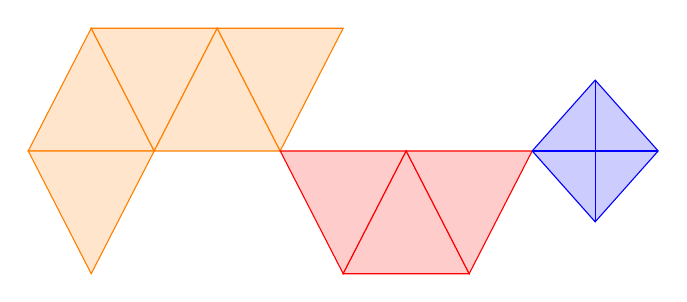
\begin{tikzpicture}[every node/.style={fill,circle,inner sep=1.5pt},yscale=0.9,xscale=0.8]

  % Define the coordinates for the shared vertices of orange triangles
  \coordinate (P1) at (0,0);
  \coordinate (P2) at (2,0);
  \coordinate (P3) at (1,1.732); % height of equilateral triangle
  \coordinate (P4) at (3,1.732);

  % Draw the orange triangles
  \filldraw[orange, fill=orange!20] (P1) -- (P2) -- (P3) -- cycle; % 1st triangle
  \filldraw[orange, fill=orange!20] (P2) -- (P3) -- (P4) -- cycle; % 2nd triangle
  \coordinate (P5) at (4,0); % Shift for the 3rd triangle
  \filldraw[orange, fill=orange!20] (P2) -- (P4) -- (P5) -- cycle; % 3rd triangle
  \coordinate (P6) at (5,1.732); % Height for the 4th triangle
  \filldraw[orange, fill=orange!20] (P4) -- (P5) -- (P6) -- cycle; % 4th triangle
  \coordinate (P7) at (1,-1.732);
  \filldraw[orange, fill=orange!20] (P1) -- (P2) --(P7) -- cycle;

  % Define the coordinates for the red triangles
  \coordinate (R1) at (5,-1.732);
  \coordinate (R2) at (6,0); 
  \coordinate (R3) at (7,-1.732);

  % Draw the red triangles
  \filldraw[red, fill=red!20] (P5) -- (R1) -- (R2) -- cycle; % 1st red triangle
  \filldraw[red, fill=red!20] (R2) -- (R1) -- (R3) -- cycle; % 2nd red triangle

  % The 3rd red triangle
  \coordinate (R4) at (8,0);
  \filldraw[red, fill=red!20] (R2) -- (R3) -- (R4) -- cycle;

  % Draw the 4-clique to the right
  \coordinate (C1) at (8,0); % Shared with 3rd red triangle
  \coordinate (C2) at (9,1);
  \coordinate (C3) at (9,-1);
  \coordinate (C4) at (10,0);
  \filldraw[blue, fill=blue!20] (R4) -- (C1) -- (C2) -- (C4) -- (C3) -- (C1); % Edges of 4-clique
  \draw[blue] (C2) -- (C3); % Diagonal of 4-clique
  \draw[blue] (C4) -- (C1); % Connect 3rd red triangle to 4-clique

  % Draw vertices of 4-clique
  % \foreach \i in {1,...,4}{
  %   \fill (C\i) circle [radius=2pt];
  % }
  % \fill (P1) circle [radius=2pt];
  % \fill (P2) circle [radius=2pt];
  % \fill (P3) circle [radius=2pt];
  % \fill (P4) circle [radius=2pt];
  % \fill (P5) circle [radius=2pt];
  % \fill (P6) circle [radius=2pt];
  % \fill (R1) circle [radius=2pt];
  % \fill (R2) circle [radius=2pt];
  % \fill (R3) circle [radius=2pt];
  % \fill (R4) circle [radius=2pt];
  % \fill (R5) circle [radius=2pt];
  
\end{tikzpicture}
         \caption{An example of hypergraph $H$. Triangles filled with colors represent hyperedges in $\hG$. Two hyperedges are 2-connected if they share two nodes. Different 2-connected components are marked in different colors. }
\label{fig:2-connectivity-H}
% \vspace{12mm}
\end{minipage}%
\hfill
\begin{minipage}{.45\textwidth}
\centering
   % \resizebox{0.7\textwidth}{!}{
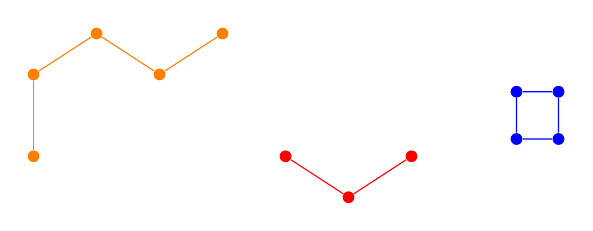
\begin{tikzpicture}[,yscale=0.9,xscale=0.8]
  % Nodes
    % Define the coordinates for the shared vertices of orange triangles
  \coordinate (P1) at (0,0);
  \coordinate (P2) at (2,0);
  \coordinate (P3) at (1,1.732); % height of equilateral triangle
  \coordinate (P4) at (3,1.732);
  \coordinate (P5) at (4,0);
  \coordinate (P6) at (5,1.732);
  \coordinate (P7) at (1,-1.732);

    % Define the coordinates for the red triangles
  \coordinate (R1) at (5,-1.732);
  \coordinate (R2) at (6,0); 
  \coordinate (R3) at (7,-1.732);

    % Draw the 4-clique to the right
  \coordinate (C1) at (8,0); % Shared with 3rd red triangle
  \coordinate (C2) at (9,1);
  \coordinate (C3) at (9,-1);
  \coordinate (C4) at (10,0);
  \coordinate (C5) at (9,0);

  \node (b1) at (barycentric cs:P1=1,P2=1,P3=1) [circle, fill=orange, inner sep=1.5pt] {};
  \node (b2) at (barycentric cs:P2=1,P3=1,P4=1) [circle, fill=orange, inner sep=1.5pt] {};
  \node (b3) at (barycentric cs:P2=1,P4=1,P5=1) [circle, fill=orange, inner sep=1.5pt] {};
  \node (b4) at (barycentric cs:P4=1,P5=1,P6=1) [circle, fill=orange, inner sep=1.5pt] {};
  \node (b5) at (barycentric cs:P1=1,P2=1,P7=1) [circle, fill=orange, inner sep=1.5pt] {};

  % Draw lines between adjacent orange barycenters
  \draw[orange] (b1) -- (b2);
  \draw[orange] (b2) -- (b3);
  \draw[orange] (b3) -- (b4);
  \draw[orange] (b1) -- (b5);

  \node (br1) at (barycentric cs:P5=1,R1=1,R2=1) [circle, fill=red, inner sep=1.5pt] {};
  \node (br2) at (barycentric cs:R2=1,R1=1,R3=1) [circle, fill=red, inner sep=1.5pt] {};
  \node (br3) at (barycentric cs:R2=1,R3=1,C1=1) [circle, fill=red, inner sep=1.5pt] {};
  \draw[red] (br1) -- (br2) -- (br3);

    \node (bc1) at (barycentric cs:C1=1,C2=1,C5=1) [circle, fill=blue, inner sep=1.5pt] {};
  \node (bc2) at (barycentric cs:C2=1,C4=1,C5=1) [circle, fill=blue, inner sep=1.5pt] {};
  \node (bc3) at (barycentric cs:C3=1,C4=1,C5=1) [circle, fill=blue, inner sep=1.5pt] {};
  \node (bc4) at (barycentric cs:C3=1,C1=1,C5=1) [circle, fill=blue, inner sep=1.5pt] {};
  \draw[blue] (bc1) -- (bc2) -- (bc3) -- (bc4) -- (bc1);
\end{tikzpicture}
         \caption{The corresponding graph $\cG_H$. Each node in $\cG_H$ corresponds to a hyperedge in $H$. Two nodes are connected if their corresponding hyperedges share two nodes.}
         % \label{fig:three sin x}
     % \end{subfigure}
% \caption{An example of  2-connectivity and 2-connected components when $d=3$.}
\label{fig:2-connectivity-G}
\end{minipage}
\end{figure}

\begin{figure}
     \centering
     \begin{subfigure}[t]{0.48\textwidth}
         \centering
         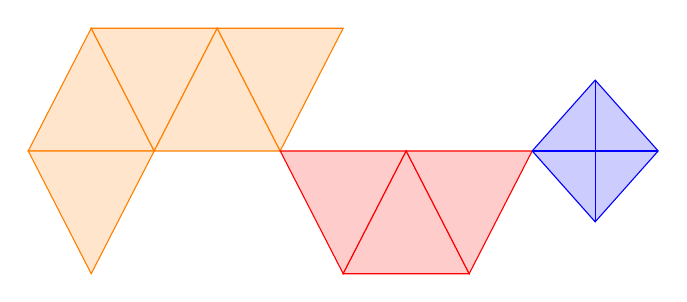
\begin{tikzpicture}[every node/.style={fill,circle,inner sep=1.5pt},yscale=0.9,xscale=0.8]

  % Define the coordinates for the shared vertices of orange triangles
  \coordinate (P1) at (0,0);
  \coordinate (P2) at (2,0);
  \coordinate (P3) at (1,1.732); % height of equilateral triangle
  \coordinate (P4) at (3,1.732);

  % Draw the orange triangles
  \filldraw[orange, fill=orange!20] (P1) -- (P2) -- (P3) -- cycle; % 1st triangle
  \filldraw[orange, fill=orange!20] (P2) -- (P3) -- (P4) -- cycle; % 2nd triangle
  \coordinate (P5) at (4,0); % Shift for the 3rd triangle
  \filldraw[orange, fill=orange!20] (P2) -- (P4) -- (P5) -- cycle; % 3rd triangle
  \coordinate (P6) at (5,1.732); % Height for the 4th triangle
  \filldraw[orange, fill=orange!20] (P4) -- (P5) -- (P6) -- cycle; % 4th triangle
  \coordinate (P7) at (1,-1.732);
  \filldraw[orange, fill=orange!20] (P1) -- (P2) --(P7) -- cycle;

  % Define the coordinates for the red triangles
  \coordinate (R1) at (5,-1.732);
  \coordinate (R2) at (6,0); 
  \coordinate (R3) at (7,-1.732);

  % Draw the red triangles
  \filldraw[red, fill=red!20] (P5) -- (R1) -- (R2) -- cycle; % 1st red triangle
  \filldraw[red, fill=red!20] (R2) -- (R1) -- (R3) -- cycle; % 2nd red triangle

  % The 3rd red triangle
  \coordinate (R4) at (8,0);
  \filldraw[red, fill=red!20] (R2) -- (R3) -- (R4) -- cycle;

  % Draw the 4-clique to the right
  \coordinate (C1) at (8,0); % Shared with 3rd red triangle
  \coordinate (C2) at (9,1);
  \coordinate (C3) at (9,-1);
  \coordinate (C4) at (10,0);
  \filldraw[blue, fill=blue!20] (R4) -- (C1) -- (C2) -- (C4) -- (C3) -- (C1); % Edges of 4-clique
  \draw[blue] (C2) -- (C3); % Diagonal of 4-clique
  \draw[blue] (C4) -- (C1); % Connect 3rd red triangle to 4-clique

  % Draw vertices of 4-clique
  % \foreach \i in {1,...,4}{
  %   \fill (C\i) circle [radius=2pt];
  % }
  % \fill (P1) circle [radius=2pt];
  % \fill (P2) circle [radius=2pt];
  % \fill (P3) circle [radius=2pt];
  % \fill (P4) circle [radius=2pt];
  % \fill (P5) circle [radius=2pt];
  % \fill (P6) circle [radius=2pt];
  % \fill (R1) circle [radius=2pt];
  % \fill (R2) circle [radius=2pt];
  % \fill (R3) circle [radius=2pt];
  % \fill (R4) circle [radius=2pt];
  % \fill (R5) circle [radius=2pt];
  
\end{tikzpicture}
         \caption{An example of hypergraph $H$. Triangles filled with colors represent hyperedges in $\hG$. Two hyperedges are 2-connected if they share two nodes. Different 2-connected components are marked in different colors. }
     \end{subfigure}
     \hfill
     \begin{subfigure}[t]{0.48\textwidth}
         \centering
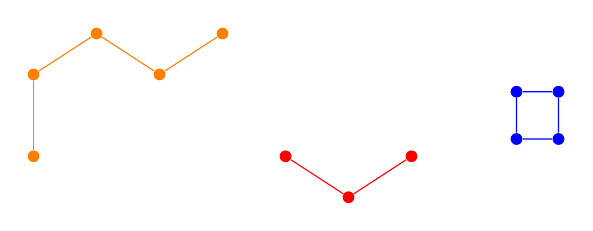
\begin{tikzpicture}[,yscale=0.9,xscale=0.8]
  % Nodes
    % Define the coordinates for the shared vertices of orange triangles
  \coordinate (P1) at (0,0);
  \coordinate (P2) at (2,0);
  \coordinate (P3) at (1,1.732); % height of equilateral triangle
  \coordinate (P4) at (3,1.732);
  \coordinate (P5) at (4,0);
  \coordinate (P6) at (5,1.732);
  \coordinate (P7) at (1,-1.732);

    % Define the coordinates for the red triangles
  \coordinate (R1) at (5,-1.732);
  \coordinate (R2) at (6,0); 
  \coordinate (R3) at (7,-1.732);

    % Draw the 4-clique to the right
  \coordinate (C1) at (8,0); % Shared with 3rd red triangle
  \coordinate (C2) at (9,1);
  \coordinate (C3) at (9,-1);
  \coordinate (C4) at (10,0);
  \coordinate (C5) at (9,0);

  \node (b1) at (barycentric cs:P1=1,P2=1,P3=1) [circle, fill=orange, inner sep=1.5pt] {};
  \node (b2) at (barycentric cs:P2=1,P3=1,P4=1) [circle, fill=orange, inner sep=1.5pt] {};
  \node (b3) at (barycentric cs:P2=1,P4=1,P5=1) [circle, fill=orange, inner sep=1.5pt] {};
  \node (b4) at (barycentric cs:P4=1,P5=1,P6=1) [circle, fill=orange, inner sep=1.5pt] {};
  \node (b5) at (barycentric cs:P1=1,P2=1,P7=1) [circle, fill=orange, inner sep=1.5pt] {};

  % Draw lines between adjacent orange barycenters
  \draw[orange] (b1) -- (b2);
  \draw[orange] (b2) -- (b3);
  \draw[orange] (b3) -- (b4);
  \draw[orange] (b1) -- (b5);

  \node (br1) at (barycentric cs:P5=1,R1=1,R2=1) [circle, fill=red, inner sep=1.5pt] {};
  \node (br2) at (barycentric cs:R2=1,R1=1,R3=1) [circle, fill=red, inner sep=1.5pt] {};
  \node (br3) at (barycentric cs:R2=1,R3=1,C1=1) [circle, fill=red, inner sep=1.5pt] {};
  \draw[red] (br1) -- (br2) -- (br3);

    \node (bc1) at (barycentric cs:C1=1,C2=1,C5=1) [circle, fill=blue, inner sep=1.5pt] {};
  \node (bc2) at (barycentric cs:C2=1,C4=1,C5=1) [circle, fill=blue, inner sep=1.5pt] {};
  \node (bc3) at (barycentric cs:C3=1,C4=1,C5=1) [circle, fill=blue, inner sep=1.5pt] {};
  \node (bc4) at (barycentric cs:C3=1,C1=1,C5=1) [circle, fill=blue, inner sep=1.5pt] {};
  \draw[blue] (bc1) -- (bc2) -- (bc3) -- (bc4) -- (bc1);
\end{tikzpicture}
         \caption{The corresponding graph $\cG_H$. Each node in $\cG_H$ corresponds to a hyperedge in $H$. Two nodes are connected if their corresponding hyperedges share two nodes.}
         \label{fig:three sin x}
     \end{subfigure}
\caption{An example of  2-connectivity and 2-connected components when $d=3$.}
\label{fig:2-connectivity}
\end{figure}


\subsubsection{Decomposition of MAP Across 2-Connected Components}

The following lemma implies that the task of finding the minimum preimage \emph{decomposes} and can be carried out individually in each of the 2-connected components of hyperedges. 


Recall that the clique hypergraph $\cliG$ (defined at the start of Section~\ref{sec:maxclique}) of a graph $G=(V,E)$ has hyperedge set $\cli(E) = \b\{\he\in \textstyle{\binom{[n]}{d}} : (i,j)\in E
\text{ for every } \{i,j\}\subset h
\b\}$.

\begin{lemma}\label{lem:union-min-preimage}
Let $C_1,\cdots, C_m$ be all 2-connected components (i.e., 2-connected subsets of hyperedges) of the clique hypergraph $\cliG$ of the projected graph $G_p=([n],E_p)$. We have
\[
\prim(\pG) = \{\cup_{i=1}^m\hG_i: \hG_i\in \prim(\proj(C_i))\}.
\]
In words, any preimage of $\pG$ is given by a union of hypergraphs, each from a preimage of the projection of a 2-connected component of $\cliG$.
% We abuse notation and use $\proj^{-1}(H)$ to denote $\proj^{-1}(\proj(H))$. 
    % The set of preimages of $\pG$ is given by the union of the preimages of \nbyp{projections of} every 2-connected component of $\cliG$.

    % \nbyp{This is really poorly phrased, because what you mean is that you have to select different preimages for different components. Just remove the statement of the Lemma and make the statement be the first paragraph (including the display) of the proof.}
\end{lemma}
The proof of the lemma is given in Appendix~\ref{sec:union-min-preimage}. 
% \red{YP: don't you want to say instead that the pre-image is given by a Cartesian product of pre-images of components?}\cg{CG: I think we need to say that it is the union of the preimages of components, not just a tuple of preimages}

What makes this decomposition so useful is that with high probability each of the components is of constant size. This will allow us to carry out a brute-force search on each component. 

\begin{restatable}{lemma}{component}\label{lem:component-constant-size}
     For any fixed $\delta<\frac{d-1}{d+1}
     % =:\tcth
     $, with high probability, all 2-connected components of $\cliG$ have size at most $1+2^{d+1}/(\frac{d-1}{d+1}-\delta)=O_n(1)$.
\end{restatable}
% \cg{Give a name for the threshold and add an illustration.}

% \red{
We will refer to this threshold, $\tcth$, as the \emph{\cth}. 
% It will play an important role in our analysis.
% }
% \cg{We didn't prove 2-connectivity of the entire graph above the threshold, so the name might be misleading.}

\subsubsection{MAP Algorithm}
% In the next section, we will show that when $\delta<\frac{d-1}{d+1}$, with high probability all 2-connected components are of constant size. This gives us 
We have the following efficient algorithm that (with high probability) implements the MAP rule $\cA^*$:
\begin{algorithm}\caption{Maximum a Posteriori (MAP) $\cA^*$}\label{alg:map}
\begin{algorithmic}[1]
\State Input: $\pG = ([n],\pE)$
\State Calculate the clique graph $\cliG$ from $\pG$ by finding all size-$d$ cliques in $\pG$.
\State Enumerate over all pairs of vertices to determine 2-neighborhoods of all hyperedges in $\cliG$.
\State Find all 2-connected components of $\cliG$ using a depth-first search on all hyperedges in $\cliG$.
\State Search over all preimages in each 2-connected components of $\cliG$ and find one with minimum size. 
\State Output the union of the minimum preimages of the 2-connected components in $\cliG$.
\end{algorithmic}
\end{algorithm}

% \begin{algorithm}\caption{Maximum a Posteriori (MAP) $\cA^*$}\label{alg:map}
% \begin{algorithmic}[1]
% \STATE Input: $\pG = ([n],\pE)$.
% \STATE Calculate the clique graph $\cliG$ from $\pG$ by finding all size-$d$ cliques in $\pG$.
% \STATE Enumerate over all pairs of vertices to determine 2-neighborhoods of all hyperedges in $\cliG$.
% \STATE Find all 2-connected components of $\cliG$ using depth first search on all hyperedges in $\cliG$.
% \STATE Search over all preimages in each 2-connected components of $\cliG$ and find one with minimum size. 
% \STATE Output the union of minimum preimages of all 2-connected components in $\cliG$.
% \end{algorithmic}
% \end{algorithm}

% This gives us an efficient algorithm for MAP.

\begin{proof}[Proof of Theorem~\ref{thm:sparse-algo}]
From the previous section, we know that MAP returns an arbitrary minimum preimage of the projected graph $\pG$. By Lemma~\ref{lem:union-min-preimage}, a minimum preimage of $\pG$ is given by the union of minimum preimages of all 2-connected components in $\cliG$. So Algorithnm~\ref{alg:map} indeed implements the MAP rule.

% This gives us the following procedure of calculating MAP:
% \begin{enumerate}
%     \item Calculate the clique graph $\cliG$ from $\pG$ by finding all size-$d$ cliques in $\pG$.
%     \item Find all 2-connected components of $\cliG$ by union-find algorithm.
%     \item Search over all possible preimages in each 2-connected components of $\cliG$ and find the one with minimum size. 
%     \item Output the union of minimum preimages of all 2-connected components in $\cliG$.
% \end{enumerate}
We now analyze the running time of the algorithm. Steps 2 and 4 take time at most $O_n(n^d)$. Step 3 takes time at most $O_n(n^2)$. 
Step 5 takes time at most $n^d2^k$, where $k$ is the size of the largest 2-connected component in $\cliG$. By Lemma~\ref{lem:component-constant-size}, $k=O_n(1)$ with high probability, so overall the algorithm finishes in time $O_n(n^d)$ with high probability.
% \cg{If we are careful about how the hyperedges are represented, and use list instead of a tensor, we can improve the running time to be $f(d)n^{g(\delta)}\le f(d)n^{3}$. This requires an extra bound on the number of inclusions. Not sure if this worth writing up. Maybe put in the appendix}\cg{Maybe mention that time complexity blows up when $\delta$ approaches the branching threshold}
\end{proof}

\subsubsection{2-Connected Components have Constant Size for Sparse Hypergraphs}\label{sec:const-size}
In this section we give a proof sketch of Lemma~\ref{lem:component-constant-size} which states that $\cliG$ can be partitioned into small 2-connected components for $\delta$ below $\frac{d-1}{d+1}$. 
We give the full proof in Section~\ref{sec:growth-components}.


The lemma is proved by carefully examining how a set of 2-connected edges in $\cliG$ can grow bigger. This is analogous to (but  more delicate than) the analysis of components in subcritical Erd\H os-R\'enyi graphs.  We will show that any 2-connected component can be decomposed into a series of ``growth'' steps starting from a single hyperedge. Each growth operation has a ``probabilistic cost" because it is a moderately low probability event, which reduces the number of such components. Accounting for the possible growth patterns within 2-connected components in $\cliG$ shows that with high probability no large components appear. 

Now let us consider the possible ways to grow a sub-hypergraph $\shG\subset \rhG$ via local exploration, and try to understand why the probability of having the graph in $\cliG$ decreases with the growth. Suppose $\shG$ is a set of hyperedges, and $\cli(\proj(\shG))$ is 2-connected. For $\shG$ to get larger, it must include one of its 2-neighbors $\he\in \cliG$. How did $\he$ appear in $\cliG$? The somewhat delicate aspect of this is that $\he$ may not be in $\rhG$: $\he$ might exist in $\cliG$ because all edges in the clique $\proj(\he)$ are covered by \emph{some other} hyperedges $\hE\subset \rhG$. So to grow $\shG$, one option is to include all of $\hE$. 
Because each hyperedge is included with fairly small probability, this reduces the expected number of components of the given form, while the number of options in selecting $\hE$ increases with the size of $\hE$. The following lemma gives
the expected number of appearances of a given sub-hypergraph $\shG$ in terms of the number of nodes and the number of hyperedges in the sub-hypergraph.  

% \cg{Should we put the definition of grow here? It's also needed later in the description of the algorithm. We can make more precise claims but the definition is very complicated.}

% Lemma~\ref{lem:number-appearance} states that 

\begin{lemma}\label{lem:number-appearance} Let $X_{\shG}$ be the number of appearances of a sub-hypergraph $\shG$ in $\rhG$. Denote by $v_\shG$ and $e_\shG$ the number of nodes and hyperedges in $\shG$.
    For any hypergraph $\shG$, 
    \[
    \E X_{\shG} = \Theta_n(n^{v_\shG}p^{e_\shG})\,.
    \]
\end{lemma}
When we grow $\shG$, we increase both the number of nodes and the number of edges of the hypergraph. With more nodes, the expectation increases (more possible choices) and with more hyperedges, the expectation decreases. The trade-off is controlled by how we choose $\hE$ and the parameter $\delta$. When $\delta<\frac{d-1}{d+1}$, we will be able to show that no matter how $\hE$ is chosen, the expectation always decreases by a polynomial factor. Therefore, after a constant number of growth steps, the expectation becomes negligible.

% \cg{Here $H$ (and ambiguous graph in the next section) refers to a copy of a sub-hypergraph, so the vertex set is not on $[n]$ but on a small number of vertices in a different space. Do we want a separate notation for subgraphs and sub-hypergraphs? Also strictly we should say the number of subgraphs in $\rhG$ that is isomorphic to $H$ instead of the number of appearances of sub-hypergraph $H$.}

% \cg{
% I think right now the statement is intuitive, as $H$ do serve as possible sub-hypergraphs. But technically it is not a specific sub-hypergraph but refers to all possible copies.}
\subsection{Ambiguous Graphs and Success Probability of MAP}
In this section, we will see that when $\delta $ is below the \cth\  $\tcth$, the success probability of MAP is fully determined by graphs with non-unique minimum preimages, which we call ambiguous graphs.

\begin{definition}\label{def:ambiguous}
    An \emph{ambiguous graph} is a graph with at least two minimum hypergraph preimages.
\end{definition}


As we will see, appearance or non-appearance of ambiguous graphs determines success of the MAP rule. 

\subsubsection{Impossibility Result via Existence 
 of Ambiguous Graphs}
 
In the previous section, we showed that MAP is w.h.p. efficient whenever $\delta<\frac{d-1}{d+1}$. However, even the optimal algorithm does not always succeed in this regime. Consider the graph depicted in Figure~\ref{fig:ambiguous-graph}. If $\pG$ has a copy of this graph as a component, then there are two minimum preimages with equal size, both with the same posterior probability. So no matter which one the MAP algorithm outputs, it must incur at least 1/2 probability of error. This is formalized in the following lemma.


\begin{figure}

   \begin{minipage}{0.48\textwidth}\centering
   % \resizebox{0.45\textwidth}{!}{
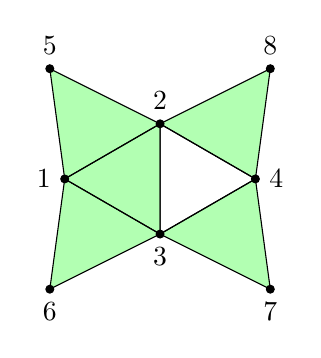
\begin{tikzpicture}[node/.style={minimum size = 1mm, inner sep=0pt}, scale=0.7]
    % Define vertices of the triangles
    \coordinate (1) at (-1.73,0);
    \coordinate (2) at (0,1);
    \coordinate (3) at (0,-1);
    \coordinate (4) at (1.73,0);
    \coordinate (5) at (-2,2);
    \coordinate (6) at (-2,-2);
    \coordinate (7) at (2,-2);
    \coordinate (8) at (2,2);

    
    \fill[green!30] (1) -- (2) -- (3) -- cycle;
    \fill[green!30] (1) -- (2) -- (5) -- cycle;
    \fill[green!30] (1) -- (3) -- (6) -- cycle;
    \fill[green!30] (4) -- (2) -- (8) -- cycle;
    \fill[green!30] (4) -- (7) -- (3) -- cycle;

    % Draw triangles
    \draw (1) -- (2) -- (3) -- cycle;
    \draw (2) -- (3) -- (4) -- cycle;
    \draw (1) -- (2) -- (5) -- cycle;
    \draw (1) -- (3) -- (6) -- cycle;
    \draw (2) -- (4) -- (8) -- cycle;
    \draw (3) -- (4) -- (7) -- cycle;

    % Label vertices
    \node at (1) [draw, circle, fill=black, scale=0.5,inner sep=2pt, label=left:1] {};
    \node at (2) [draw, circle, fill=black, scale=0.5,inner sep=2pt, label=above:2] {};
    \node at (3) [draw, circle, fill=black, scale=0.5,inner sep=2pt, label=below:3] {};
    \node at (4) [draw, circle, fill=black, scale=0.5,inner sep=2pt, label=right:4] {};
    \node at (5) [draw, circle, fill=black, scale=0.5,inner sep=2pt, label=above:5] {};
    \node at (6) [draw, circle, fill=black,scale=0.5, inner sep=2pt, label=below:6] {};
    \node at (7) [draw, circle, fill=black, scale=0.5,inner sep=2pt, label=below:7] {};
    \node at (8) [draw, circle, fill=black, scale=0.5,inner sep=2pt, label=above:8] {};

\end{tikzpicture}
    % \caption{A graph with non-unique minimum preimage when $d=3$. Green hyperedges are the two possible minimum preimages.}
    % \label{fig:ambiguous-graph}
% \end{figure}
\end{minipage}\hfill
   \begin{minipage}{0.48\textwidth}\centering

% \begin{figure}
% \centering
% % \begin{subfigure}{}
% % \end{subfigure}
% % \hfill
% \begin{subfigure}
% \centering
   % \resizebox{0.45\textwidth}{!}{
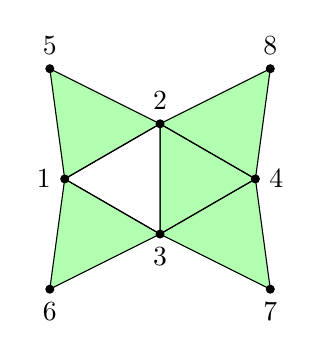
\begin{tikzpicture}[node/.style={minimum size = 0mm, inner sep=0pt}, scale=0.7]
    % Define vertices of the triangles
    \coordinate (1) at (-1.73,0);
    \coordinate (2) at (0,1);
    \coordinate (3) at (0,-1);
    \coordinate (4) at (1.73,0);
    \coordinate (5) at (-2,2);
    \coordinate (6) at (-2,-2);
    \coordinate (7) at (2,-2);
    \coordinate (8) at (2,2);

    
    \fill[green!30] (4) -- (2) -- (3) -- cycle;
    \fill[green!30] (1) -- (2) -- (5) -- cycle;
    \fill[green!30] (1) -- (3) -- (6) -- cycle;
    \fill[green!30] (4) -- (2) -- (8) -- cycle;
    \fill[green!30] (4) -- (7) -- (3) -- cycle;

    % Draw triangles
    \draw (1) -- (2) -- (3) -- cycle;
    \draw (2) -- (3) -- (4) -- cycle;
    \draw (1) -- (2) -- (5) -- cycle;
    \draw (1) -- (3) -- (6) -- cycle;
    \draw (2) -- (4) -- (8) -- cycle;
    \draw (3) -- (4) -- (7) -- cycle;

    % Label vertices
    \node at (1) [draw, circle, fill=black,scale=0.5, inner sep=2pt, label=left:1] {};
    \node at (2) [draw, circle, fill=black,scale=0.5, inner sep=2pt, label=above:2] {};
    \node at (3) [draw, circle, fill=black,scale=0.5, inner sep=2pt, label=below:3] {};
    \node at (4) [draw, circle, fill=black,scale=0.5, inner sep=2pt, label=right:4] {};
    \node at (5) [draw, circle, fill=black,scale=0.5, inner sep=2pt, label=above:5] {};
    \node at (6) [draw, circle, fill=black,scale=0.5, inner sep=2pt, label=below:6] {};
    \node at (7) [draw, circle, fill=black,scale=0.5, inner sep=2pt, label=below:7] {};
    \node at (8) [draw, circle, fill=black,scale=0.5, inner sep=2pt, label=above:8] {};

\end{tikzpicture}
% }
% \end{subfigure}

\end{minipage}
\caption{A graph with non-unique minimum preimage in the case $d=3$. The green hyperedges are the two possible minimum preimages.}
\label{fig:ambiguous-graph}
\end{figure}

\begin{restatable}{lemma}{badgraphinisolation}\label{lem:bad-graph-in-isolation}
    For any ambiguous graph $G_a$ and any recovery algorithm $\cA$, given input $\pG = \proj(\rhG)$,
    \[
    \Pr(\cA(\pG)\ne\rhG) \ge \frac{1}{2}\Pr\b(\cli(G_a)\text{ is a 2-connected component of }\cliG \b)\,.
    \]
\end{restatable}

% \begin{lemma}\label{lem:bad-graph-in-isolation}

% \end{lemma}
\begin{proof}
By Lemma~\ref{lem:union-min-preimage}, a minimum preimage of $\pG$ is given by the union of the minimum preimages of every 2-connected component of $\cliG$. Therefore, when $\cli(G_a)$ is a 2-connected component of $\cliG$, the minimum preimage of $\cliG$ is not unique. So no matter which hypergraph $\cA^*$ chooses, it has at least 1/2 probability of making a mistake. In other words,
\[
\Pr(\cA(\pG)\ne\rhG|\cli(G_a)\text{ is a 2-connected component of }\cliG) \ge 1/2\,.
\]
The lemma follows from Bayes rule. 
\end{proof}

It follows that to prove impossibility of (exact) recovery, we only need to find an ambiguous graph that is a 2-connected component with probability $\Omega_n(1)$.
% \cg{Define ambiguous graph threshold}
Let the \emph{ambiguity threshold}, $\ath$, be the infimum of $\delta$ such that there exists an ambiguous graph appearing as a 2-connected component with probability $\Omega_n(1).$
\[
\ath \defeq \inf\{\delta:\exists G_a, \Pr(\cli(G_a)\text{ is a 2-connected component of }\cliG) = \Omega_n(1) \}\,.
\]
It then follows from Lemma~\ref{lem:bad-graph-in-isolation} that exact recovery is impossible for any $\delta$ that is at least $\ath$. 
% In other words, $\cdel d \le \ath$.
% \red{
In other words, we have the following corollary.
\begin{corollary}\label{cor:critical-threshold-smaller-ambiguous-threshold}
    For any $d$, we have $\cdel d \le \ath\,.$
\end{corollary}
% }


This will allow us to prove the impossibility results in Theorem~\ref{thm:main-three} and Theorem~\ref{thm:main-four-five} showing that $\ath$, and hence also $\cdel d$, is at most $\frac{2d-4}{2d-1}$ when $d\le 5$.  The construction of the ambiguous graph will be described in Section~\ref{sec:impossibility}. It will be a generalization of Figure~\ref{fig:ambiguous-graph} to general $d$.


This approach stops working for $d\ge 6$. In Section~\ref{sec:impossibility}, we will show that the regime of $\delta$ in which such an ambiguous graph appears as a 2-connected component in $\rhG$ is between $\frac{2d-4}{2d-1}$ and the \cth\ $\frac{d-1}{d+1}$. When $d\ge 6$, $\frac{2d-4}{2d-1}$ is above the \cth\ and the ambiguous graph typically overlaps with other hyperedges, i.e., it does not appear as a component. In this case it is no longer clear that there are at least two equally likely preimages.

We next work towards understanding
when a given sub-hypergraph will appear in $\rhG$.

\subsubsection{Appearance of Sub-hypergraphs in Random Hypergraphs}

We will need a lemma that determines the threshold density for a given graph to appear in the random $d$-hypergraph, $\rhG(n,d,p)$.
The graph version of the lemma was first proven in \cite{bollobas1981threshold} and simplified in \cite{rucinski1986strongly}. For random hypergraphs, the proof is similar and we include it in Appendix~\ref{sec:subgraph_threshold} for completeness.
\begin{lemma}\label{lem:subgraph_threshold}
    For a hypergraph $\shG = (V,\hE_\shG)$,
    define \[
    m(\shG) = \max_{\shG'\subset \shG}\frac{e_{\shG'}}{v_{\shG'}}\,,
    \]
    % where $\shG[V']$ is the induced subgraph on $V'$ and $e$ denotes the number of hyperedges in the subgraph. 
    where $e_{\shG'}$ and $v_{\shG'}$ are the number of edges and the number of nodes of sub-hypergraph $\shG$.
    We have
    \[
    \Pr(\shG\subset \rhG) = 
    \begin{cases}
        o_n(1) &\text{if }p=o_n(n^{-1/m(\shG)})\\
        1-o_n(1) &\text{if }p=\omega_n(n^{-1/m(\shG)})\\
        \Omega_n(1) &\text{if } p =\Theta_n(n^{-1/m(\shG)}).
    \end{cases}
    \]
\end{lemma}


\subsubsection{Reconstruction Result by Nonexistence of Ambiguous Graphs}\label{sec:main-idea-reconstruction}
In this section we prove the following theorem.
\begin{theorem}\label{thm:delta-lower}
    When $d=3$ and $\delta<2/5$ or when $d=4,5$ and $\delta<1/2$, the MAP rule achieves exact recovery and moreover it can be implemented efficiently.
\end{theorem}
In the regime where $\delta<
% \tcth=
\frac{d-1}{d+1}$, which is the regime we care about when $d\le 5$, the converse of Lemma~\ref{lem:bad-graph-in-isolation} is also true. That is, if with high probability no ambiguous graph (i.e., with non-unique minimum cover) appears in $\pG$ as a 2-connected component, then MAP succeeds with high probability.

\begin{lemma}\label{lem:no-ambiguous}
    Assume $\delta<
    % \tcth=
    \frac{d-1}{d+1}$.
    If for all finite ambiguous graphs $G_a$,
    \[
    \Pr\b(\cli(G_a)\text{ is a 2-connected component of }\cliG \b)=o_n(1)\,,
    \]
    % $\Pr(G_a\subset \pG)=o_n(1)$
    % with at most $\frac{d(2^d+1)}{\frac{d-1}{d+1}-\delta} $ vertices 
    % with non-unique minimum cover 
    then we have 
    \[
    \Pr(\cA^*(\pG)=\rhG)\ge 1- o_n(1)\,.
    \]
\end{lemma}
% \cg{Define the ambiguous graph threshold. Explain here the relation between the two thresholds.}

The lemma is proved in Appendix~\ref{sec:proof-no-ambiguous}. 
Here we provide a sketch of the proof. If there is no ambiguous graph in $\pG$, the projections of every 2-connected components have a unique minimum preimage. As shown in Lemma~\ref{lem:component-constant-size}, all 2-connected components are of constant size. Under this condition, the minimum preimage of the 2-connected component is correct with probability $1-O_n(p)$, as any other preimage is $O_n(p)$ times less likely in the posterior and there are only constant number of possible preimages. The overall minimum preimage, as given by $\cA^*$, is then correct with high probability by union bound over all 2-connected components.

% \red{
Recall the definition of the ambiguous threshold, $\ath$, Lemma~\ref{lem:no-ambiguous} implies that the critical threshold $\cdel d$ is above $\ath$ if $\ath$ is below $\tcth$.
\begin{corollary}
    For any $d$, if $\ath\le\tcth$, we have $ \cdel d \ge \ath$.
\end{corollary}

Combining this corollary with Corollary~\ref{cor:critical-threshold-smaller-ambiguous-threshold}, we get that the ambiguous threshold $\ath$ fully determines the critical threshold $\cdel d$ if $\ath$ is below $\tcth$.
\begin{corollary}
    For any $d= 3,4,5$, we have $\ath\le\tcth$, and hence $ \cdel d = \ath$.
\end{corollary}
% }
\begin{figure}
    \centering
    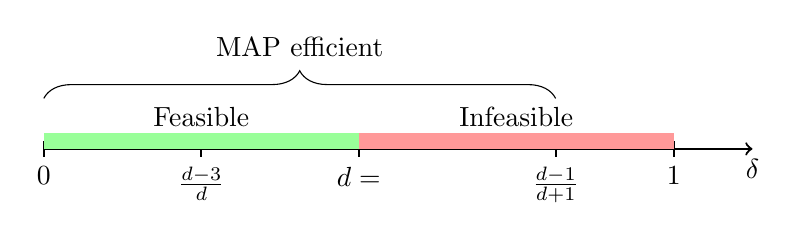
\begin{tikzpicture}
    % Draw the main axis
    \draw[thick, ->] (-4,0) -- (5,0) node[anchor=north] {$\delta$};

    % Draw and label the first threshold
    \draw[thick] ({-2},0.1) -- ({-2},-0.1) node[below] {$\frac{d-3}{d}$};

    % Draw and label the second threshold (ambiguous threshold)
    \draw[thick] (0,0.1) -- (0,-0.1) node[below] {$\cdel d = \ath$};

    % Draw and label the third threshold (2-connectivity threshold)
    \draw[thick] (2.5,0.1) -- (2.5,-0.1) node[below] {$
    % \tcth=
    \frac{d-1}{d+1}$};

    % Add additional ticks and labels as needed
    \foreach \x in {0,1}
        \draw[thick] (8*\x-4,0.1) -- (8*\x-4,-0.1) node[below] {\x};

        % Color the regions
    % Feasible region: from 0 to the ambiguous threshold (green)
    \fill[green!40] (-4,0) rectangle (0.4,0.2);
    \node at (-2,0.4) {Feasible};

    % Infeasible region: from the ambiguous threshold to 1 (red)
    \fill[red!40] (0,0) rectangle (4,0.2);
    \node at (2,0.4) {Infeasible};

    % Add curly brace to indicate region from 0 to 2-connectivity threshold
    \draw [decorate,decoration={brace,amplitude=10pt,raise=4pt},yshift=0pt]
    (-4,0.5) -- (2.5,0.5) node [black,midway,yshift=0.8cm] {MAP efficient};
\end{tikzpicture}
    \caption{
    % \gb{make a second figure with them swapped somehow explaining why for $d\geq 6$ things are different}
    % \red{
    Relation between different thresholds. The maximum clique cover algorithm $\cliA$ succeeds with high probability up to $\delta=\frac{d-3}{d}$. The MAP algorithm is efficient up to $\tcth$ and succeeds with high probability up to threshold $\cdel d$. If $\ath<\tcth$, then $\cdel d$ is the same as the ambiguous threshold $\ath$.
    % }
    }
    \label{fig:thresholds-relation}
\end{figure}

As long as we can check the condition in Lemma~\ref{lem:no-ambiguous} for a specific $\delta$, MAP is optimal. If $\delta<\tcth$, then with high probability all 2-connected components have size bounded by $(2^d+1)/(\frac{d-1}{d+1}-\delta)$, so there are only finitely many graphs we need to check. This gives us the following computer assisted method of proving that MAP works when $\delta $ is below a hypothesized threshold $\delta_0$:
\begin{enumerate}
    \item Enumerate over all hypergraphs $\shG$ with at most $1+2^{d+1}/(\frac{d-1}{d+1}-\delta_0)$ hyperedges.
    \item Compute the probability that $\shG\subset \rhG$ by Lemma~\ref{lem:subgraph_threshold} with $p=n^{-d+1+\delta_0}$.
    % (deferred due to space constraints). 
    \item Enumerate all possible preimages of $\proj(\shG)$ and see if $\proj(\shG)$ is ambiguous.
    \item If all graphs are either not ambiguous or have vanishing probability of occurring, the condition in Lemma~\ref{lem:no-ambiguous} is satisfied and MAP succeeds with high probability at $\delta=\delta_0$.
\end{enumerate}
Since $\Pr(\shG\subset \rhG)$ monotonically increases with $\delta$, we know the same condition holds for any $\delta<\delta_0$.

Although this approach can be carried out in principle, the number of hypergraphs with at most $1+2^{d+1}/(\frac{d-1}{d+1}-\delta_0)$ hyperedges is a huge number and cannot be verified in reasonable time. Instead of doing a brute force search, we will utilize the structure of how 2-connected components grow, as discussed in Section~\ref{sec:const-size}, to reduce the runtime. The runtime of the search can be further reduced by identifying properties of ambiguous graph and focusing on graphs with such properties. 

With the computer search, we are able to prove the following lemma. The search algorithm will be discussed in more detail in Section~\ref{sec:algo-proof}.
\begin{restatable}{lemma}{lowerbound}\label{lem:delta-lowerbound}
    When $d=3$ and $\delta<2/5$ or when $d=4,5$ and $\delta<1/2$, any ambiguous graph $G_a$ 
    % of size at most $2\binom{d}{2}/\b({\frac{d-1}{d+1}-\delta} \b)$
    satisfies
    $
    \Pr(G_a\subset \pG)=o_n(1).
    $
\end{restatable}

Combining this lemma and Lemma~\ref{lem:no-ambiguous} completes the proof of Theorem~\ref{thm:delta-lower}.
% \begin{proof}[proof of Theorem~\ref{thm:delta-lower}]
% Follows directly from Lemma~\ref{lem:no-ambiguous} and Lemma~\ref{lem:delta-lowerbound}.
% \end{proof}
\subsection{Upper Bound on $\cdel d$ for Large $d$ and Proof of Theorem~\ref{thm:main-large-d}}
We identify a sufficient condition for the (optimal) MAP rule to fail:
Suppose there is a hyperedge $\he$ in $\rhG$ where every pair of nodes in $\he$ is also included in other hyperedges in $\rhG$. In this case the graph $\rhG\setminus \{\he\}$ has higher probability and has the same graph projection. 
Because the optimal algorithm outputs a minimum preimage, it does not output the original hypergraph $\rhG$: deleting $\he$ forms a smaller preimage.

We formalize this sufficient condition and consider a hypergraph $\bG$ with the following hyperedges:
\begin{itemize}
    \item $\{v_1,\cdots,v_d\}$,
    \item $\{v_i,v_j,u_{ij}^{(1)}, u_{ij}^{(2)},\cdots, u_{ij}^{(d-2)}\}$ for all $\{i,j\}\subset [d] $, where for each $i$ and $j$ the nodes $u_{ij}^{(1)}, u_{ij}^{(2)},\cdots, u_{ij}^{(d-2)}$ are arbitrary.
\end{itemize}

From the discussion above, we know that $\cA^*$ will fail if $\bG\subset\rhG$, because the hyperedge $v_1,\cdots,v_d$ can be removed from the output and increase the posterior probability. 
% 
Therefore, we have
\[
\Pr(\cA^*(\pG)\ne \rhG) \ge \Pr(\bG\subset\rhG)\,.
\]
By Lemma~\ref{lem:subgraph_threshold}, this occurs with probability $\Omega_n(1)$ when $p=\Omega_n(n^{-1/m(\bG)})$. Since 
\[
m(\bG) = \frac{e_{\bG}}{v_{\bG}} = \frac{\binom{d}{2}+1}{d+\binom{d}{2}(d-2)}\,,
\]
this is equivalent to 
\[
p=\Omega_n(n^{-d\frac{d^2-3d+4}{d^2-d+2}})\,,
\]
or $\delta\ge \frac{d^2-d-2}{d^2-d+2}$.
We have shown the following impossibility result:
\begin{theorem}\label{thm:large-d}
    Exact recovery is information theoretically impossible when  $\delta\ge \frac{d^2-d-2}{d^2-d+2}$\,.
\end{theorem}

% \red{
% \begin{itemize}
%     \item We ask the basic question of when does projecting a hypergraph to a graph losses information, equivalently, when is it possible to recover the original hypergraph from a projected graph.
%     \item Inspiration from social network and biology. How to recover higher order interactions from a graph.
%     \item Some data are inherently hypergraph, but treated as a graph. Examples from social science. 
%     \item We want to understand when is projecting hypergraph to a normal graph a good strategy to develop algorithms. The answer depends on specific question of interest, but we can gain insight by studying the fundamental limit of when the projection start to loss information.
%     \item The same question has been studied from empirical point of view and tested on real data sets.
%     \item To understand the question in theory, we study random hypergraphs, as worst-case hypergraphs is impossible to recover.
%     \item Definition of the problem
%     \item We obtain tight bounds of exact recovery for random $d$-hypergraph when $d=3,4,5$.
%     \item An interval for $d\ge 6$? We can have some simple upper and lower bounds.
%     \item A chart for the results.
% \end{itemize}
% }




% \subsection{Maximum Clique Cover Algorithm}
\label{sec:maxclique}
When the graph is so sparse that each hyperedge appears as an isolated clique, exact recovery is easily achieved by creating a hypergraph with a hyperedge for every clique of the projected graph $\pG$. This algorithm turns out to succeed far beyond the regime where hyperedges do not overlap.
% \cg{This might be a good place to introduce the clique graph}


Let the \emph{$d$-clique hypergraph }$\cliG$ of the projected graph $\pG=([n], E_p)$ be the hypergraph $\cliG = ([n],\cliE=\cli(\pE))$ where
\[
\cli(E) = \b\{\he\in \textstyle{\binom{[n]}{d}} : (i,j)\in E
\text{ for every } \{i,j\}\subset h
\b\}\,.
\]
% We use $\Ic(\he)$ to be the indicator that a hyperedge $\he$ is included in $\cliG$.
% It is easy to see that any $\hE\in \prim(E)$ is a subset of $\cli(E)$. 
% \cg{cg: only retain what is really used below}
% Notice that there is a bijection between all possible $d$-clique hypergraphs and the image set of $\proj$, as $\proj(\cli(E))=E$. 
% When we say the minimum preimage or the minimum cover of a $d-$clique hypergraph, we refer to the minimum preimage or the minimum cover of the corresponding projected graph.
% 
Denote by $\cliA$ the algorithm converting every size-$d$ clique in $\pG $ to a hyperedge in the output graph, i.e., $\cliA(\pG) = \cli(\pE)$. We call this the \emph{maximum clique cover algorithm}.

% \begin{algorithm}\caption{Maximum Clique Cover Algorithm $\cliA$}\label{alg:clique-cover}
% \begin{algorithmic}[1]
% \STATE Input: $\pG = ([n],\pE)$
% \STATE  $\cli(\pE)\leftarrow \emptyset$
% \FOR{all size $d$ subsets of $[n]$}
%     \STATE If $\pE$ has a clique on the subset, add the hyperedge on the subset to $\cli(\pE)$
% \ENDFOR
% \STATE Output $\cli(\pE)$
% \end{algorithmic}
% \end{algorithm}

\begin{algorithm}\caption{Maximum Clique Cover Algorithm $\cliA$}\label{alg:clique-cover}
\begin{algorithmic}[1]
\State Input: $\pG = ([n],\pE)$
\State  $\cli(\pE)\leftarrow \emptyset$
\For {all size $d$ subsets of $[n]$}
    \State If $\pE$ has a clique on the subset, add the hyperedge on the subset to $\cli(\pE)$
\EndFor
\State Output $\cli(\pE)$
\end{algorithmic}
\end{algorithm}

\begin{remark}
    Since we are enumerating all size-$d$ subsets, the algorithm has time complexity $n^d$. It may be possible to improve this runtime by taking advantage of sparsity of the graph, using ideas in \cite{boix2021average}. 
\end{remark}


For which parameters does this algorithm work? 
% Unfortunately, this does not reach the optimal threshold. 
From the definition, $\cliA$ fails if and only if there exists a clique in $\pG$ that is not a hyperedge of $\rhG$. 
If a $d$-clique $\he$ in $\pG$ is not a hyperedge of $\rhG$, every edge in the clique is included in some other hyperedge $\he'\in \rhG$. By carefully examining the possible ways of inclusion for all edges, we can obtain a tight bound on the probability of the event, yielding the following threshold.

% \gbdone{why is this $d-1$ in denom while Theorem 1.3 has $d$?}
% \cg{It should be $d$, this is a typo.}
\begin{theorem}\label{thm:naive}
    $\cliA$ exactly recovers $\rhG$ when $\delta< \frac{d-3}{d}$ and has $\Omega_n(1)$ probability of failure when $\delta\ge \frac{d-3}{d}$.
\end{theorem}
This implies the positive recovery  result in Theorem~\ref{thm:main-large-d} for $d\geq 6$, which we believe to be suboptimal. The proof of Theorem~\ref{thm:naive} is in Appendix~\ref{sec:naive}. 
% 


\subsection{Greedy Algorithm}
Another natural algorithm starts with the maximum clique cover algorithm and then greedily deletes redundant hyperedges from the clique graph.


\begin{algorithm}\caption{Greedy Algorithm}\label{alg:greedy}
\begin{algorithmic}[1]
\State Input: $\pG = ([n],\pE)$
\State Find the $d$-clique hypergraph $H_0\leftarrow\cli(\pE)$
\While{$\exists h\in H_0$ that $H_0\backslash h\in \proj^{-1}(\hE_\rhG)$}
    \State $H_0\leftarrow H_0\backslash h$
\EndWhile
\State Output $H_0$
\end{algorithmic}
\end{algorithm}

% \begin{algorithm}\caption{Greedy Algorithm}\label{alg:greedy}
% \begin{algorithmic}[1]
% \STATE Input: $\pG = ([n],\pE)$
% \STATE Find the $d$-clique hypergraph $H_0\leftarrow\cli(\pE)$
% \WHILE{$\exists h\in H_0$ that $H_0\backslash h\in \proj^{-1}(\hE_\rhG)$}
%     \STATE $H_0\leftarrow H_0\backslash h$
% \ENDWHILE
% \STATE Output $H_0$
% \end{algorithmic}
% \end{algorithm}

% \begin{enumerate}
%     \item Find the $d$-clique hypergraph $H_0\leftarrow\cli(\pE)$.
%     \item Delete a hyperedge from $H_0$ if after the deletion the graph is still in $\proj^{-1}(\hE_\rhG)$. Repeat until all hyperedge cannot be deleted.
%     \item Output $H_0$
% \end{enumerate}

Heuristically this algorithm ought to work better than the maximum clique cover algorithm, because it yields a graph with higher posterior probability. We leave it as an open question to determine under which parameter regime this algorithm succeeds. 
% \cg{Is there more we can say this algorithm? An alternative choice is to put this in open problem session.}

\section{Preliminaries}
\label{Preliminaries}
\subsection{Multi-Agent Reinforcement Learning}
A MARL problem can be formulated as a decentralized partially observed Markov decision process (Dec-POMDP)~\cite{oliehoek2016concise}, which is described as a tuple $\langle n,\boldsymbol{S},\boldsymbol{A},P,R,\boldsymbol{O},\boldsymbol{\Omega},\gamma\rangle $, where $n$ represents the number of agents, $\boldsymbol{S}$ is the global state space. $\boldsymbol{A}$ is the action space. $\boldsymbol{O}=\{O_{i}\}_{i=1,\cdots,n}$ is the observation space. At timestep $t$, each agent $i$ receives an observation $o_{i}^t\in O_{i}$ according to the observation function $\boldsymbol{\Omega}(s^t,i):\boldsymbol{S}\to O_i$ and then selects an action $a_i^t\in\boldsymbol{A}$. The joint action $\boldsymbol{a}^t=(a_1^t,\ldots,a_n^t)$ is then applied to the environment, resulting in a transition to the next state $s^{t+1}$ and a global reward signal $r^{t}$ according to the transition function $P(s^{t+1}\mid s^{t},\boldsymbol{a}^t)$ and the reward function $R(s^t,\boldsymbol{a}^t)$. $\gamma\in[0,1]$ is the discount factor. The objective is to learn a joint policy $\pi$ that maximizes the expected cumulative reward $\mathbb{E}\left[\sum_{t=0}^{\infty}\gamma^{t}r^{t}\right|\pi]$.

\subsection{Centralized Training With Decentralized Execution}
Centralized Training with Decentralized Execution (CTDE) is a commonly employed architecture in MARL~\cite{lowe2017multi,rashid2020monotonic}. In CTDE, each agent utilizes an actor network to make decisions based on local observations. Additionally, the training process incorporates global information to train a centralized value function. The centralized value function provides a centralized gradient to update the actor network based on its outputs.

\subsection{Generalizable Model Structure in MARL}
To handle varying state/observation/action spaces, previous works like UPDeT~\cite{hu2021updet} and ASN~\cite{wang2019action} propose a generalizable model that treats all agents as entities. In such models, observation $o_i$ can be conducted as entity-observations: $[o_{i,1},o_{i,2},...,o_{i,m}]$, where $m$ denotes the number of all entities in the environment. Based on the criterion of whether entites can be observed, entity-observations can be splited into two subsets: observed entity-observations $o_{\mathrm{obs},i}$ and unobserved entity-observations $o_{\mathrm{mask},i}$. We denote the number of observed entities and masked entities as $n_{\mathrm{obs}}$ and $n_{\mathrm{mask}}$, respectively, and it holds that $m=n_{\mathrm{obs}}+n_{\mathrm{mask}}$.
Additionally, action space $\boldsymbol{A}$ can be decomposed into two subsets:$\boldsymbol{A}^{\mathrm{self}}$ containing actions that affect the environment or itself  and $\boldsymbol{A}^{\mathrm{out}}$ representing actions that directly interact with other entities.

\section{Threshold of Growth for 2-Connected Components}\label{sec:growth-components}
In this section we prove that for sparse hypergraphs, all 2-connected components have constant size.
\component*

In order to prove the lemma, we formalize the notion of growing a subhypergraph.

\paragraph{Possible 2-neighbors of a sub-hypergraph and Definition of $\grow$.}
In Section~\ref{sec:const-size}, we discussed that the size of 2-connected components can be bounded by examining how 2-connected sub-hypergraphs can grow. Specifically, we will look at a sub-hypergraph $H\subset \rhG$ and the possible ways for $H$ to have a 2-neighbor. 
% \red{check all uses}
% \gb{What's happening here?}



Suppose $\shG$ is a sub-hypergraph of $\rhG$ and $\cli(\proj(\shG))$ is 2-connected. 
Let $N(\shG)$ 
% $N(\shG)\defeq \nei{\chG d}(\cli(\proj(\shG)))$ 
be the set of all possible 2-neighbors of $\cli(\proj(\shG))$. If $\cli(\proj(\shG))$ is a proper subset of a larger 2-connected hypergraph $\cli(\proj(\shG'))$ for some $\shG'\subset \rhG$, then there must exist $\he \in N(\shG)$ that is in $\cli(\proj(\shG'))$. An example is drawn in Figure~\ref{fig:possible-neighbors}, where $\shG$ only contains one hyperedge $\{1,2,3\}$, and all 3 possible 2-neighbors of $\{1,2,3\}$ forms $N(\shG)$.
% \begin{figure}
% \centering
% \begin{tikzpicture}
%     \coordinate (1) at (0,0);
%     \coordinate (2) at (4,0);
%     \coordinate (3) at (2,3.46);
%     \coordinate (4) at (2,-3.46);
%     \coordinate (5) at (-2,3.46);
%     \coordinate (6) at (6,3.46);
%     % Main triangle 123 in the middle

%     % Fill triangle 123 with green
%     \fill[green!30] (1.center) -- (2.center) -- (3.center) -- cycle;
%     \fill[cyan!30] (1.center) -- (2.center) -- (4.center) -- cycle;
%     \fill[cyan!30] (1.center) -- (3.center) -- (5.center) -- cycle;
%     \fill[cyan!30] (3.center) -- (2.center) -- (6.center) -- cycle;
%     \node[draw, circle, fill=black, label=left:1] (1) at (0,0) {};
%     \node[draw, circle, fill=black, label=right:2] (2) at (4,0) {};
%     \node[draw, circle, fill=black, label=above:3] (3) at (2,3.46) {}; % 3.46 approximates sqrt(12) to form an equilateral triangle
    
%     % Additional nodes 4, 5, 6
%     \node[draw, circle, fill=black, label=below:4] (4) at (2,-3.46) {}; % Placed symmetrically below 1
%     \node[draw, circle, fill=black, label=left:5] (5) at (-2,3.46) {}; % Placed symmetrically left of 2
%     \node[draw, circle, fill=black, label=right:6] (6) at (6,3.46) {}; % Placed symmetrically right of 3
    
%     % Dotted line triangles 124, 235, and 136
%     % \draw[dotted] (1) -- (2) -- (4) -- (1);
%     % \draw[dotted] (2) -- (3) -- (6) -- (2);
%     % \draw[dotted] (1) -- (3) -- (5) -- (1);
% \end{tikzpicture}
% \caption{An illustration of $N(\hE)$. Here $\hE$ only has one hyperedge $\{1,2,3\}$, colored in green. $N(\hE)$ contains three possible 2-neighbors of $\cli(\proj(\hE))=\hE$, colored in blue.}
% \label{fig:possible-neighbors}
% \end{figure}

\begin{figure}
\centering
\begin{minipage}{.45\textwidth}

\centering
   % \resizebox{0.7\textwidth}{!}{
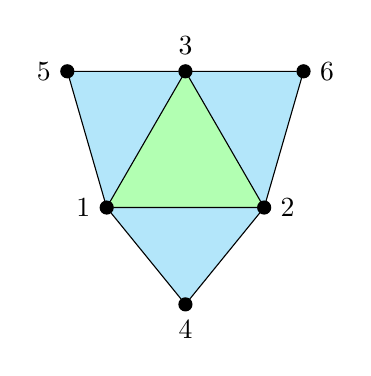
\begin{tikzpicture}[scale=0.50]
    \coordinate (1) at (0,0);
    \coordinate (2) at (4,0);
    \coordinate (3) at (2,3.46);
    \coordinate (4) at (2,-2.46);
    \coordinate (5) at (-1,3.46);
    \coordinate (6) at (5,3.46);
    % Main triangle 123 in the middle

    % Fill triangle 123 with green
    \fill[green!30] (1.center) -- (2.center) -- (3.center) -- cycle;
    \fill[cyan!30] (1.center) -- (2.center) -- (4.center) -- cycle;
    \fill[cyan!30] (1.center) -- (3.center) -- (5.center) -- cycle;
    \fill[cyan!30] (3.center) -- (2.center) -- (6.center) -- cycle;
    \node[draw, circle, fill=black, scale=0.5,label=left:1] (1) at (0,0) {};
    \node[draw, circle, fill=black, scale=0.5,label=right:2] (2) at (4,0) {};
    \node[draw, circle, fill=black, scale=0.5,label=above:3] (3) at (2,3.46) {}; % 3.46 approximates sqrt(12) to form an equilateral triangle
    
    % Additional nodes 4, 5, 6
    \node[draw, circle, fill=black, scale=0.5,label=below:4] (4) at (4) {}; % Placed symmetrically below 1
    \node[draw, circle, fill=black, scale=0.5,label=left:5] (5) at (5) {}; % Placed symmetrically left of 2
    \node[draw, circle, fill=black, scale=0.5,label=right:6] (6) at (6) {}; % Placed symmetrically right of 3
    
    \node at (barycentric cs:1=1,2=1,3=1) {$\shG$};
    
    % Dotted line triangles 124, 235, and 136
    \draw (1) -- (2) -- (4) -- (1);
    \draw (2) -- (3) -- (6) -- (2);
    \draw (1) -- (3) -- (5) -- (1);
\end{tikzpicture}
\caption{An illustration of $N(\shG)$ when $d=3$. Here $\shG$ only has one hyperedge $\{1,2,3\}$, colored in green. $N(\shG)$ contains three possible 2-neighbors of $\cli(\proj(\shG))=\shG$, colored in blue.}
\label{fig:possible-neighbors}
\vspace{12mm}
\end{minipage}%
\hfill
\begin{minipage}{.45\textwidth}
\centering
   % \resizebox{0.7\textwidth}{!}{
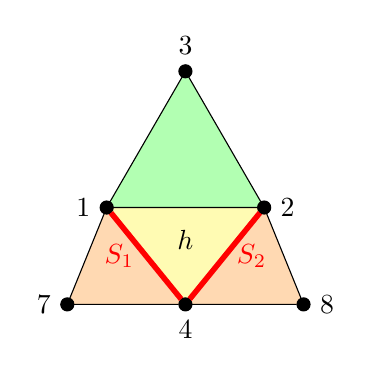
\begin{tikzpicture}[scale=0.50]
    % Define coordinates
    \coordinate (1) at (0,0);
    \coordinate (2) at (4,0);
    \coordinate (3) at (2,3.46);
    \coordinate (4) at (2,-2.46);
    % \coordinate (5) at (-2,3.46);
    % \coordinate (6) at (6,3.46);
    \coordinate (7) at (-1,-2.46); % Additional point to the left
    \coordinate (8) at (5,-2.46); % Additional point to the right
    
    % Fill triangles with respective colors
    \fill[green!30] (1.center) -- (2.center) -- (3.center) -- cycle;
    \fill[yellow!30] (1.center) -- (2.center) -- (4.center) -- cycle; % Refill with yellow
    % \fill[cyan!30] (1.center) -- (3.center) -- (5.center) -- cycle;
    % \fill[cyan!30] (3.center) -- (2.center) -- (6.center) -- cycle;
    \fill[orange!30] (1.center) -- (4.center) -- (7.center) -- cycle; % New triangle 147
    \fill[orange!30] (2.center) -- (4.center) -- (8.center) -- cycle; % New triangle 248
    
    % Draw nodes
    \node[draw, circle, fill=black,scale=0.5, label=left:1] (1) at (1) {};
    \node[draw, circle, fill=black, scale=0.5,label=right:2] (2) at (2) {};
    \node[draw, circle, fill=black, scale=0.5,label=above:3] (3) at (3) {};
    \node[draw, circle, fill=black, scale=0.5,label=below:4] (4) at (4) {};
    % \node[draw, circle, fill=black, label=left:5] (5) at (5) {};
    % \node[draw, circle, fill=black, label=right:6] (6) at (6) {};
    \node[draw, circle, fill=black,scale=0.5, label=left:7] (7) at (7) {};
    \node[draw, circle, fill=black, scale=0.5, label=right:8] (8) at (8) {};
    
    % Dotted line triangles
    \draw (1) -- (2) -- (4) -- (1);
    % \draw (2) -- (3) -- (6) -- (2);
    % \draw (1) -- (3) -- (5) -- (1);
    \draw (1) -- (4) -- (7) -- (1); % Dotted lines for new triangle 147
    \draw (2) -- (4) -- (8) -- (2); % Dotted lines for new triangle 248
    
    % Place "h" in the middle of triangle 124
    \node at (barycentric cs:1=1,2=1,4=1) {$h$};
    \node at (barycentric cs:1=1,2=1,3=1) {$\shG$};
    
    % Color intervals 14 and 24 and add labels
    \draw[line width=2pt, red] (1) -- node[left] {$S_1$} (4);
    \draw[line width=2pt, red] (2) -- node[right] {$S_2$} (4);
    
    % Draw edges for clarity (optional)
    \draw (1) -- (2);
    \draw (1) -- (3);
    \draw (2) -- (3);
\end{tikzpicture}
\caption{An example of an element in $\grow(\shG,\he)$, consists of 3 hyperedges, $\{1,2,3\},\{1,4,7\}\text{ and }\{2,4,8\}$. Here $\shG$ contains one hyperedge $\{1,2,3\}$. $\he=\{1,2,4\}$. For $\he$ to be included in the 2-connected component, one way is to include $S_1^{\shG,\he} = \{1,4\}$ and $S_2^{\shG,\he} = \{2,4\}$ respectively in two hyperedges. }
\label{fig:example-grow}
\end{minipage}
\end{figure}

For $\he\in N(\shG)$ to appear in the 2-connected hypergraph $\cli(\proj(\shG'))$, every edge in $\proj(\he)\backslash \proj(\shG)$ should be covered in at least one hyperedge in $\shG'$.
Now let us examine the possible ways for this to happen.  
Let $\cS^{\shG,\he} \defeq \{S_1^{\shG,\he}, S_2^{\shG,\he}, \cdots, S_m^{\shG,\he}\}$ be the collection of subsets of $\he$ such that $\proj(S_i)\not\subseteq \proj(\shG)$ and $\proj(S_i)\ne \emptyset$. Let $m$ be the number of such subsets, and note that $m\le 2^d$. 
If a hyperedge covers an edge in $\proj(\he)\backslash \proj(\shG)$, it must intersect with $h$ at one of the sets in $\cS^{\shG,\he}$. For any $\he\in N(\shG)$, we define
% \gbdone{change $K$ to $S$ and then can use $K$ later for sub-hypergraph}
\[
    \grow(\shG, \he) \defeq \{\shG\cup(\cup_{i\in I}\{\he_i\}): I\subseteq [m], \he_i\cap \he = S_i^{\shG,\he} , \proj(\cup_{i\in I}S_i^{\shG,\he}) = \proj(h)\backslash \proj(\shG)\}\,,
\]
and
\[
\grow(\shG) \defeq  \bigcup_{\he\in N(\shG)}\grow(\shG)\,.
\]
An example of an element in $ \grow(\shG, \he)$ is shown in Figure~\ref{fig:example-grow}.
% \begin{figure}
% \centering
% \begin{tikzpicture}
%     % Define coordinates
%     \coordinate (1) at (0,0);
%     \coordinate (2) at (4,0);
%     \coordinate (3) at (2,3.46);
%     \coordinate (4) at (2,-3.46);
%     \coordinate (5) at (-2,3.46);
%     \coordinate (6) at (6,3.46);
%     \coordinate (7) at (-3,-3.46); % Additional point to the left
%     \coordinate (8) at (7,-3.46); % Additional point to the right
    
%     % Fill triangles with respective colors
%     \fill[green!30] (1.center) -- (2.center) -- (3.center) -- cycle;
%     \fill[yellow!30] (1.center) -- (2.center) -- (4.center) -- cycle; % Refill with yellow
%     % \fill[cyan!30] (1.center) -- (3.center) -- (5.center) -- cycle;
%     % \fill[cyan!30] (3.center) -- (2.center) -- (6.center) -- cycle;
%     \fill[orange!30] (1.center) -- (4.center) -- (7.center) -- cycle; % New triangle 147
%     \fill[orange!30] (2.center) -- (4.center) -- (8.center) -- cycle; % New triangle 248
    
%     % Draw nodes
%     \node[draw, circle, fill=black, label=left:1] (1) at (1) {};
%     \node[draw, circle, fill=black, label=right:2] (2) at (2) {};
%     \node[draw, circle, fill=black, label=above:3] (3) at (3) {};
%     \node[draw, circle, fill=black, label=below:4] (4) at (4) {};
%     % \node[draw, circle, fill=black, label=left:5] (5) at (5) {};
%     % \node[draw, circle, fill=black, label=right:6] (6) at (6) {};
%     \node[draw, circle, fill=black, label=left:7] (7) at (7) {};
%     \node[draw, circle, fill=black, label=right:8] (8) at (8) {};
    
%     % Dotted line triangles
%     \draw[dotted] (1) -- (2) -- (4) -- (1);
%     % \draw[dotted] (2) -- (3) -- (6) -- (2);
%     % \draw[dotted] (1) -- (3) -- (5) -- (1);
%     \draw[dotted] (1) -- (4) -- (7) -- (1); % Dotted lines for new triangle 147
%     \draw[dotted] (2) -- (4) -- (8) -- (2); % Dotted lines for new triangle 248
    
%     % Place "h" in the middle of triangle 124
%     \node at (barycentric cs:1=1,2=1,4=1) {$h$};
    
%     % Color intervals 14 and 24 and add labels
%     \draw[line width=2pt, red] (1) -- node[left] {$S_1$} (4);
%     \draw[line width=2pt, red] (2) -- node[right] {$S_2$} (4);
    
%     % Draw edges for clarity (optional)
%     \draw (1) -- (2);
%     \draw (1) -- (3);
%     \draw (2) -- (3);
% \end{tikzpicture}
% \caption{An example of an element in $\grow(\hE,\he)$, consists of 3 hyperedges, $\{1,2,3\},\{1,4,7\},\{2,4,8\}$. Here $\hE$ contains one hyperedge $\{1,2,3\}$. $\he=\{1,2,4\}$. For $\he$ to be included in the 2-connected component, one way is to include $S_1^{\shG,\he} = \{1,4\}$ and $S_2^{\shG,\he} = \{2,4\}$ respectively in two hyperedges. }
% \label{fig:example-grow}
% \end{figure}

% Let $\hE_i^\he$ be the set of such hyperedges.
% \[
% \hE_i^\he\defeq \B\{\he'\in \binom{[n]}{d}: \he'\cap \he = S_i^{\shG,\he}\B\}\,
% \]
% \cg{cg: This paragraph is probably too dense.}

Any 2-connected component can be achieved by ``growing'' multiple times from a single $d$-hyperedge.
\begin{lemma}\label{lem:grow-contain-all-components}
% Let $\shG$ be a hypergraph $\cli(\proj(\shG))$ is 2-connected. 
% There exists $t\ge 0$ such that $\shG\in \grow^{(t)}([d])$. 
% In other words, 
Assume w.l.o.g. that hyperedge $[d]$ is in a given $\shG$. We have that
\[
\{\shG:\text{$\cli(\proj(\shG))$ is 2-connected}\} = \bigcup_{t\ge 0}\grow^{(t)}([d])\,,
\]
where $\grow^{(t)}$ denotes applying $\grow$ $t$ times.
% \cg{select a better expression}
% For any $\hE_1$ where $\cli(\proj(\hE_1))\supset \cli(\proj(\hE))$ is 2-connected, there exists $\hE_2\in \grow(\hE_1)$ such that  $\hE\subseteq \hE_2\subset\hE_1.$
\end{lemma}
\begin{proof}
Choose an arbitrary size-$d$ hyperedge in $\shG$, without loss of generality assume it is $[d]$. We will grow it to $\shG$ by applying $\grow$ multiple times.

Specifically, we will show that given any $\shG_1\subset \shG$, there exists $\shG_2\in \grow(\shG_1)$ such that $\shG_1\subset \shG_2\subseteq \shG$. So $\shG$ can be obtained by growing $[d]$ finite number of times, as any hypergraph in $\grow(\shG_1)$ has more hyperedges than $\shG_1$.

If $\shG_1\subset \shG$, there must exists a $\he\in N(\{\shG_1\})$ in $\cli(\proj(\shG))$. As all edges in $\proj(\he)$ are in $\proj(\shG)$, we can select a set of hyperedges $\hE$ in $\shG$ that covers all edges in $\proj(\he)\backslash \proj(\shG_1)$. 
Let $\hE_i$ be the subset of hyperedges in $\hE$ that intersect with $\he$ at $S^{\shG_1,\he}_i$ 
\[
\hE_i\defeq \{\he'\in \hE: \he' \cap \he = S^{\shG_1,\he}_i\}\,.
\]
Let $\hE'$ be a set of edges by selecting one hyperedge from each non-empty $\hE_i$. We have $\proj(\hE')\supset \proj(\he)\backslash \proj(\shG_1)$.
Therefore, 
\[
\shG_2\defeq  \shG_1\cup\hE'\in  \grow(\shG_1,\he)\,.\qedhere
\]
% Let $\hE'\subseteq \hE$ be obtained from $\hE$ by deleting hyperedges that do not intersect with $\he$ and 
\end{proof}

\paragraph{Decrease in the Expected Number of Appearances after Growth.}
To bound the probability of a large 2-connected component, we will show that any grow operation decreases the expected number of hypergraphs by a polynomial factor.

\begin{lemma}\label{lem:exp-dec}
Suppose $\delta<\frac{d-1}{d+1}$.
Let $X_\shG$ denote the number of appearance of $\shG$ in $\rhG$. Then for any $\shG$ with $O_n(1)$ number of vertices and any $\shG'\in \grow(\shG)$,
\[
\frac{\E X_{\shG'}}{\E X_{\shG}} = O_n\B(n^{-\b(\frac{d-1}{d+1}-\delta\b)}\B)\,.
\]
\end{lemma}

\begin{proof}
By Lemma~\ref{lem:number-appearance}, we have
\[
\E X_{\shG'} = \Theta_n(n^{v_{\shG'}}p^{e_{\shG'}}) \quad\text{and}\quad \E X_{\shG} = \Theta_n(n^{v_{\shG}}p^{e_{\shG}}) \,,
\]
So $\frac{\E X_{\shG'}}{\E X_{\shG}} = \Theta_n (n^{v_{\shG'}-v_{\shG}}p^{e_{\shG'}-e_{\shG'}})$. We bound this by considering all possible ways to grow $\shG$.

Suppose $\shG' \in \grow(\shG,\he)$ where $\he\in N(\shG)$. From the definition of $\grow(\shG,\he)$, let $\shG'\backslash\shG =\{\he_i\}_{i\in I}$ where
\[
\{\he_i\}_{i\in I} \text{ satisfy }   \he_i\cap \he = S_i^{\shG,\he} \text{ and } \proj(\cup_{i\in I}S_i^{\shG,\he}) = \proj(h)\backslash \proj(\shG)\,.
\] 
So $e_{\shG'}-e_{\shG'} = |I|$. The set of nodes in $\shG'$ but not in $\shG$ is given by the set of nodes that are in $\he$ but not $\shG$, which has size $d-k$, and the set of nodes that are in $\he_i$ but not in $\shG$ which has size $d-|S_i^{\shG,\he}|$. Therefore, we have
\[
v_{\shG'}-v_{\shG} \le  d-k+\sum_{i\in I} (d-|S_i^{\shG,\he}|)\,.
\]
We have inequality instead of equality because some vertices may be double-counted. 

Therefore,
\[
\begin{split}
\frac{\E X_{\shG'}}{\E X_{\shG}} &= O_n(n^{d-k+\sum_{i\in I} (d-|S_i^{\shG,\he}|)}p^{|I|})\,.
\end{split}
\]
Using $p=n^{-d+1+\delta}$, we have that for any $\shG'$,
\[
\frac{\E X_{\shG'}}{\E X_{\shG}} =O_n\B(n^{d-k}\cdot\max_{ \substack{I\subset[m]:\\(\proj(\he)\backslash \proj(\shG)) \subset \cup_i\proj(S_i^{\shG,\he})}} n^{-\sum_{i\in I}(|S_i^{\shG,\he}|-1-\delta)}\B)\,.
\]
Suppose $h$ shares $k$ nodes with $V(\shG)$. Here $k$ is at least 2 and at most $d$. 
We know $\proj(\he)\cap \proj(\shG)$ is a subset of a size-$k$ clique in $\he$. So the above expression can be further relaxed to $O_n(n^{d-k-g_k(\delta)})$ where
\begin{equation}\label{eq:gdelta}
g_k(\delta) \defeq \min_{\substack{I\subset [m]:\\ \b(\proj(\he)\backslash \binom{U_\he}{2}\b) \subset \cup_i\proj(S_i^\he)}} \sum_{i\in I}(|S_i^\he|-1-\delta)\,.
\end{equation}
Here $U_\he$ is a size-$k$ subset of $\he$. Here $g_k(\delta)$ does not depend on the choice of $\he$. We will show a a bound on $\min_k \{g_k(\delta)+k-d\}$ in Lemma~\ref{lem:cover-bound} at the end of the section. Given the bound in Lemma~\ref{lem:cover-bound}, we have for any $\delta<\frac{d-1}{d+1}$,
\[
\frac{\E X_{\shG'}}{\E X_{\shG}} = O_n\B(n^{-\b(\frac{d-1}{d+1}-\delta\b)}\B)\,.\qedhere
\]
% Further, let $S_k$ be the set of hyperedges that has $k$ nodes in $V(\hE_1)$, i.e., 
% \[
% S_k \defeq \B\{\he\in \binom{[n]}{d}: |\he\cap V(\hE)|=k\B\}\,.
% \]
%  The size of $S_k$ is at most
% \[
% |S_k|\le \binom{|V(S_k)|}{k}\binom{n}{d-k}=O_n(n^{d-k})\,.
% \]
\end{proof}

\paragraph{Bound on Component Size via Number of Growth Steps.}
Now we are ready to bound the size of 2-connected components.



\begin{proof}[Proof of Lemma~\ref{lem:component-constant-size}]
Let $t= 2(\frac{d-1}{d+1}-\delta)\inv$. 
We will show that with high probability any hypergraph in $\grow^{(t)}([d])$ does not appear in $\rhG$.
First, $X_{[d]} = \binom{n}{d}p = \Theta_n(n^{1+\delta})$. By Lemma~\ref{lem:exp-dec}, we have for any graph $\shG$ in $\grow^{(t)}([d])$,
\[
X_{\shG} =O_n\B(n^{1+\delta}\cdot n^{-t\b(\frac{d-1}{d+1}-\delta\b)}\B) = O_n(n^{\delta-1}) = o_n(1)\,.
\]
By Markov's inequality, $\Pr(\shG\subset \rhG) = o_n(1)$. There are $O_n(1)$ graphs in $\grow^{(t)}([d])$, so by the union bound,
\[
\Pr\b(\shG \subset \rhG\text{ for some } \shG \in\grow^{(t)}([d])\b) = o_n(1)\,.
\]
Note that for any $t'>t$, hypergraphs in $\grow^{(t')}([d])$ contains one of the hypergraphs in $\grow^{(t)}([d])$ and therefore do not appear with high probability.
So by Lemma~\ref{lem:grow-contain-all-components} with high probability, all 2-connected components in $\rhG$ are in 
\[
\bigcup_{i=0}^t \grow^{(t)}([d])\,.
\]
Since the grow operation increases the number of hyperedges by at most $2^d$, with high probability all 2-connected components in $\rhG$ have size at most
\[
1+t2^d
= 1+\frac{2^{d+1}}{\frac{d-1}{d+1}-\delta}\,,
\]
as stated in the lemma. 
\end{proof}


The lemma below shows a bound on $g_k(\delta)$ in \eqref{eq:gdelta} that was used in the proof of Lemma~\ref{lem:exp-dec}.
\begin{lemma}\label{lem:cover-bound}
For any $\delta\le \frac{d-1}{d+1}$,
    \[
    \min_{2\le k\le d,k\in \mathbb{Z}} \{g_k(\delta)+k-d\}\ge \frac{d-1}{d+1}-\delta\,.
    \]
\end{lemma}
\begin{proof}
Recall that \[
g_k(\delta) \defeq \min_{\substack{I\subset [m]:\\ \b(\proj(\he)\backslash \binom{U_\he}{2}\b) \subset \cup_i\proj(S_i^\he)}} \sum_{i\in I}(|S_i^\he|-1-\delta)\,.
\]
The function takes the minimum of linear functions of $\delta$, so this is a piece-wise linear function. Since every linear function has slope at most $-1$, $g_k(\delta)$ also has slope at most $-1$ in each piece.

Next we will lower bound the value of $g_k(\delta)$ by a series of relaxations on the domain of the optimization.
For any set of $\{S_i^\he\}_{i\in I}$, the union of edges is a superset of all edges in $\proj(\he)\backslash \binom{U_\he}{2}$. So 
we can get a lower bound on $g_k(\delta)$ by relaxing the set of possible $I$ to be the set of cliques with at least $\binom{d}{2}-\binom{k}{2}$  number of edges. Also each clique in the set $I$ that reaches minimum contains a unique edge, so $|I|\le \binom{d}{2}-1$.
\[
\min_{\substack{I\subset [m],|I|\le \binom{d}{2}-1:\\ \sum_{i\in I}\binom{|S_i^\he|}{2} \ge \binom{d}{2}-\binom{k}{2}}} \sum_{i\in I}(|S_i^\he|-1-\delta)
\,.
\]
Substituting $|S_i^\he|$ with $x_i$ and relaxing it to real numbers, we get another lower bound on $g_k(\delta)$:
\[
\min_{M\in \mathbb{Z}^+,M\le \binom{d}{2}-1}
\min_{\substack{x_1,x_2,\cdots, x_M\ge 2:\\ \sum_{i=1}^M\frac{x_i(x_i-1)}{2} \ge \binom{d}{2}-\binom{k}{2}} } \sum_{i=1}^M(x_i-1-\delta)
\,.
\]
So 
\[
\begin{split}
&\min_k \{g_k(\delta)+k-d\}\\
&\ge 
\min_{\substack{M\in \mathbb{Z}^+,\\ M\le \binom{d}{2}-1}}
\min_{2\le k\le d}
\min_{\substack{x_1,x_2,\cdots, x_M\ge 2:\\ \sum_{i=1}^M\frac{x_i(x_i-1)}{2} \ge \binom{d}{2}-\binom{k}{2}} } \B\{\sum_{i=1}^M(x_i-1-\delta)+k-d\B\}\\
& = 
\min_{\substack{M\in \mathbb{Z}^+,\\ M\le \binom{d}{2}-1}}
\min_{\substack{x_0,x_1,\cdots, x_M\ge 2:\\ \sum_{i=0}^M\frac{x_i(x_i-1)}{2} \ge \binom{d}{2}} }\B\{ \sum_{i=0}^M x_i - M(1+\delta)-d\B\}\,.
\end{split}
\]
Here in the equality we substituted $k$ with $x_0$.
By setting $y_i=\frac{x_i(x_i-1)}{2}$, the above can be written as 
\[
\min_{\substack{M\in \mathbb{Z}^+,\\ M\le \binom{d}{2}-1}}
\min_{\substack{y_0,y_1,\cdots, y_M\ge 1:\\ \sum_{i=0}^M y_i \ge \binom{d}{2}} }\B\{ \sum_{i=0}^M \B(\frac{1+\sqrt{1+8y_i}}{2}\B) - M(1+\delta)-d\B\}\,.
\]
For a fixed $M$, this is minimizing a concave function of $y$ over a polyhedron. So the minimum is either at a vertex or infinity. The latter is obviously not the minimum. So the minimum is at a vertex of the following polyhedron:
\[
P\defeq \B\{y:y_i\ge 1, \sum_{i=0}^M y_i \ge \binom{d}{2}\B\}\,.
\]
By symmetry of the function and $P$ under permutation of coordinates, we can consider one of the vertices without loss of generality. Let $y_0=y_1=\cdots=y_{M-1} = 1$, $y_M=\binom{d}{2}-M$, we have that the above is equal to
\[
\min_{\substack{M\in \mathbb{Z}^+,\\ M\le \binom{d}{2}-1}} \B\{ 2M-M(1+\delta)-d+  \frac{1+\sqrt{1+8(d(d-1)/2-M)}}{2}\B\}
\]
The function is concave in $M$, so the minimum is at $M=1$ or $M=\binom{d}{2}-1$. When $\delta=\frac{d-1}{d+1}$ and $M=\binom{d}{2}-1$, the function is 0. When $\delta=\frac{d-1}{d+1}$ and $M=1$,  the function is 
\[
\frac{1+\sqrt{1+8(d(d-1)/2-1)}}{2} -d +\frac{2}{d+1}
\]
One can solve that the roots of this function are $\frac{1}{2}\pm \frac{\sqrt{17}}{2}$ and when $d\ge3>\frac{1}{2}+ \frac{\sqrt{17}}{2}$, this function is always positive.
% 
Therefore, when $\delta=\frac{d-1}{d+1}$, $\min_k \{g_k(\delta)+k-d\} \ge 0$. Since this is a piece-wise function of $\delta$ with slope at most $-1$, we know for any $\delta\le \frac{d-1}{d+1}$, $\min_k \{g_k(\delta)+k-d\} \ge \frac{d-1}{d+1} -\delta$.
\end{proof}

% 
\section{MAP is Efficient for Sparse Hypergraphs}


% This allows us to output a minimum pre-image

% \begin{lemma}\label{lem:component-constant-size}
%     For any $\delta<\frac{d-1}{d+1}$, any 2-connected component of $\cliG$ has size at most $\frac{2}{\frac{d-1}{d+1}-\delta}=O_n(1)$ with high probability.
% \end{lemma}
% \begin{proof}
% For any $\he_1\in \binom{[n]}{d}$,
% let $C(\he_1)$ be the 2-connected component of $\cliG$ that contains $\he_1$ if $\he_1\in\hE_\rhG$ and $\emptyset$ otherwise. Let us control the probability that a 2-connected component grows from size $t-1$ to size $t$.
% % , we let $C(\he_1)=\emptyset$ if $\he_1\not \in \cliG$. For any $t\in\mathbb{Z}^+$,
% \[
% \begin{split}
%     &\Pr\b(|C(\he_1)|\ge t\b| |C(\he_1)|\ge t-1\b)\\
%     &=\Pr\b(\nei{\cliG}(\{\he_1,\cdots, \he_{t-1}\})\ne\emptyset \b| \exists h_1,\cdots, h_{t-1}\in\cliG \text{ s.t. }\{\he_1,\cdots, \he_{t-1}\}\text{ is 2-connected}\b)\\
%     &= \Pr\b(\nei{\cliG}(\{\he_1,\cdots, \he_{t-1}\})\ne\emptyset \b| \exists \text{a minimal cover $\hE$ of } h_1,\cdots, h_{t-1}\in\binom{[n]}{d}\text{ s.t. }   \{\he_1,\cdots, \he_{t-1}\}\text{ is 2-connected}, \hE\subset \hE_\rhG\b)
% \end{split}
% \]
% For any $t=O_n(1)$, any minimal cover of $h_1,\cdots, h_{t-1}$ also has size $O_n(1)$. So by Lemma~\ref{lem:branching}, 
% \[
% \Pr\b(|C(\he_1)|\ge t\b| |C(\he_1)|\ge t-1\b)=O_n(n^{-(\frac{d-1}{d+1}-\delta)})\,.
% \]
% So we have
% \[
% \begin{split}
% &\Pr(|C(\he_1)|\ge k)\\
% &=\Pr(\he_1\in \hE_\rhG)\prod_{t=2}^k\Pr\b(|C(\he_1)|\ge t\b| |C(\he_1)|\ge t-1\b)\\
% &=O_n(n^{-d+1+\delta}\cdot n^{-(k-1)(\frac{d-1}{d+1}-\delta)})\,.
% \end{split}
% \]
% Union bound over all $\he_1\in\binom{[n]}{d}$ and set $k=1+\frac{2}{\frac{d-1}{d+1}-\delta}$, we get 
% \[
% \Pr\B(\exists\he_1\in\binom{[n]}{d} , |C(\he_1)|\ge k\B) \le \binom{n}{d}O_n(n^{-d+1+\delta-(k-1)(\frac{d-1}{d+1}-\delta)}) = O_n(n^{\delta-1})=o_n(1)\,.
% \]
% This means any 2-connected component of $\cliG$ has size at most $k-1=\frac{2}{\frac{d-1}{d+1}-\delta}$ with probability $1-o_n(1)$.
% % Let  $\he_i$ to be a random hyperedge in $\nei{\cliG}(\{\he_0,\he_1,\cdots, \he_{i-1}$
% % We have
% % \[
% % |C(\he_0)|\ge t\Leftrightarrow \exists \he_1\in \nei{\cliG}(\he_0), \exists \he_2\in \nei{\cliG}(\{\he_0,\he_1\})\cdots, \exists \he_t\in \nei{\cliG}(\{\he_0,\he_1,\cdots, \he_{t-1}\})
% % \]
% % So 
% % \[
% % \Pr(|C(\he_0)|\ge t) = \prod_{i=1}^t \Pr(\exists \he_t\in \nei{\cliG}(\{\he_0,\he_1,\cdots, \he_{t-1}\}) | )
% % \]
% \end{proof}

\nbyp{I don't understand this lemma. It seems that $Proj(\mathcal{E}_1)$ is missing, but also what is the role of $\mathcal{E}_0$?}
\cg{rewrite this part}
\begin{lemma}\label{lem:branching}
For any $\hE_1\subset \binom{[n]}{d}$ with $|\hE_1|=O_n(1)$,
\[
    \Pr\b(\nei{\cliG}(\cli(\hE_1))\ne \emptyset | \hE_1\subset \hE_{\rhG}\b) =
    \begin{cases}
        O_n(n^{-(\frac{d-1}{d+1}-\delta)}) &\text{if }\delta<\frac{d-1}{d+1}\\
        1-\Omega_n(1) &\text{if }\delta=\frac{d-1}{d+1}
    \end{cases}
    \,.
\]


\end{lemma}


% We can show that the above bound is tight, \cg{delete}
% \begin{lemma}\label{lem:branching-tight}
%     When $\delta>\frac{d-1}{d+1}$, there exists $\hE_1\subset \binom{[n]}{d}$ such that 
%     \[
%     \Pr\b(\nei{\cliG}(\cli(\hE_1))\ne \emptyset | \hE_1\subset \hE_{\rhG}\b) = 1-o_n(1)\,.
%     \]
% \end{lemma}
\begin{proof}
% Note that the event $\nei{\cliG}(\cli(\hE_1))\ne \emptyset$ is monotonically increasing in all hyperedges, by Harris inequality, we have 
% \[
% \Pr\b(\nei{\cliG}(\cli(\hE_1))\ne \emptyset | \hE_1\subset \hE_{\rhG}, \hE_0\cap \hE_{\rhG}=\emptyset\b) \le \Pr\b(\nei{\cliG}(\cli(\hE_1))\ne \emptyset | \hE_1\subset \hE_{\rhG}\b)\,.
% \]
% In other words, we can consider the case when $\hE_0$ is empty without loss of generality. 

\end{proof}





\section{Impossibility when $d\le 5$ and $\delta \ge \frac{2d-4}{2d-1}$}\label{sec:impossibility}
% MAP is optimal in the sense that it succeeds with the highest probability among all possible recovery algorithms. But it still might not achieve exact recovery if the failure probability does not vanish. 

Recall that in Lemma~\ref{lem:bad-graph-in-isolation}, we reduced the problem of proving impossibility of exact recovery to finding ambiguous graphs. 
\badgraphinisolation*
In this section we will identify an appropriate ambiguous graph and then use Lemma~\ref{lem:bad-graph-in-isolation} to prove the following theorem.
\begin{theorem}\label{thm:upper}
    When $d=3,4,5$, for any $\delta\ge \frac{2d-4}{2d-1}$, exact recovery is information theoretically impossible.
\end{theorem}
% We will use the following Lemma to characterize a sufficient condition of when does any algorithm fail on exact recovery.
% \begin{lemma}\label{lem:bad-graph-in-isolation}
%     For any constant-size graph $G_a$ with non-unique minimum preimage, and any recovery algorithm $\cA$,
%     \[
%     \Pr(\cA(\pG)\ne\rhG) \ge \frac{1}{2}\Pr(\cli(G_a)\text{ is a 2-connected component of }\cliG )
%     \]
% \end{lemma}
% \begin{proof}
% By Lemma~\ref{lem:union-min-preimage}, a minimum preimage of $\pG$ is given by the union of the minimum preimages of every 2-connected component of $\cliG$. Therefore, when $\cli(G_a)$ is a 2-connected component of $\cliG$, the minimum preimage of $\cliG$ is not unique. So no matter which hypergraph $\cA^*$ chooses, it has at least 1/2 probability of making mistake. In other words,
% \[
% \Pr(\cA(\pG)\ne\rhG|\cli(G_a)\text{ is a 2-connected component of }\cliG) \ge 1/2\,.
% \]
% The lemma follows from Bayes rule. 
% \end{proof}
\subsection{Ambiguous Graph and Its Properties}

Let us list the properties we need for an ambiguous graph $\aG$ to prove the theorem:
\begin{enumerate}
    \item The graph should be ambiguous, i.e., it should have at least two minimum preimages. We will prove this property in Lemma~\ref{lem:bad-graph-non-unique-preimage}. 
    \item The graph appears in $\pG$ with constant probability, $\Pr(\aG\subset \pG)=\Omega_n(1)$. We will prove this  property in Lemma~\ref{lem:bad-graph-contain-probability}.
    \item The graph appears as a 2-connected component in $\cliG$ with constant probability.
    % \\ $\Pr(\cli(\aG)\text{ is a 2-connected component of }\cliG)=\Omega_n(1).$ 
    We will prove this property in Corollary~\ref{cor:bad-graph-probability}.
\end{enumerate}

Recall that ambiguous graph was defined in Defn.~\ref{def:ambiguous}. We will construct a specific such graph.

\begin{definition}[Ambiguous Graph $\aG$]\label{def:aG}
   We define the graph $\aG$ as the union of the following $2d$ cliques:
\begin{itemize}
    \item the clique $u_1,v_1,v_2,\cdots, v_{d-1}$, denoted by $\he_1$,
    \item the clique $u_2,v_1,v_2,\cdots, v_{d-1}$, denoted by $\he_2$,
    \item for any $1\le i\le d-1$, the clique $u_1,v_i,w_i^{(1)},w_i^{(2)},\cdots, w_i^{(d-2)}$, denoted by $\he_i^w$,
    \item and for any $1\le i\le d-1$, the clique $u_1,v_i,z_i^{(1)},z_i^{(2)},\cdots, z_i^{(d-2)}$, denoted by $\he_i^z$.
\end{itemize}
Let $S_1 = \{\he_1^w,\cdots, \he_{d-1}^w\}$ and $S_2 = \{\he_1^z,\cdots, \he_{d-1}^z\}$. See Figure~\ref{fig:ambiguous-graph} for a drawing of the graph when $d=3$. The intuition is to create a set of size $d-1$, $v_1,v_2,\cdots, v_{d-1}$ ($\{2,3\}$ in Figure~\ref{fig:ambiguous-graph}), that can be assigned to two possible hyperedges, both yielding a minimum preimage. 
\end{definition}


Now we prove that this graph satisfies the properties stated above.

\subsection{$\aG$ Satisfies Three Desired Properties}

\paragraph{Property 1: The Graph $\aG$ is Ambiguous.}
 This is shown in the following lemma.
\begin{lemma}\label{lem:bad-graph-non-unique-preimage}
 The graph $\aG$ from Defn.~\ref{def:aG} has two minimum preimages (so it is ambiguous).
\end{lemma}
\begin{proof}
Any preimage of $\aG$ must contain hyperedges in $S_1$ and $S_2$ as each $w_i^{(j)}$ ($z_i^{(j)}$) is only included in one clique. To include edges among $v_1,v_2,\cdots, v_{d-1}$, either $\he_1$ or $\he_2$ needs to be included in the preimage. Both $S_1\cup S_2\cup \{\he_1\}$ and $S_1\cup S_2\cup \{\he_2\}$ are valid preimages, so both are minimum preimages for $\aG$.
\end{proof}

\paragraph{Property 2: The Graph $\aG$ Appears with Probability $\Omega_n(1).$}
The next lemma shows that $\aG$ appears in $\pG$ with non-negligible probability using Lemma~\ref{lem:subgraph_threshold}.
\begin{lemma}\label{lem:bad-graph-contain-probability}
Let $\aG$ be as in Defn.~\ref{def:aG}. For any $ \delta\ge \frac{2d-4}{2d-1}$, 
    \[
    \Pr(\aG\subset \pG)=\Omega_n(1)\,.
    \]
\end{lemma}

\begin{proof}
Let us focus on one possible cover of $\aG$, $S_1\cup S_2\cup \{\he_1\}$,
\[
\Pr(\aG\subset \pG)\ge \Pr(S_1\cup S_2\cup \{\he_1\}\subset \hE_\rhG)\,.
\]
Recall in Lemma~\ref{lem:subgraph_threshold}, the probability of a hypergraph $\shG$ appear as a subgraph of $\rhG$ is described by  
\[
m(\shG) = \max_{\shG'\subset \shG}\frac{e_{\shG'}}{v_{\shG'}}\,.
\]
To use Lemma~\ref{lem:subgraph_threshold}, we need to calculate $m(S_1\cup S_2\cup \{\he_1\})$. The calculation is given in the following lemma.
\begin{lemma}\label{lem:density_bad_graph}
Let $S_1,S_2$, and $h_1$ be as in the Defn.~\ref{def:aG} of graph $G_{a,d}$ above. Then
% We calculate the value of function $m$ for the preimage $S_1\cup S_2\cup \{\he_1\}$ of the ambiguous graph $\aG $ in this lemma.
    \[m(S_1\cup S_2\cup \{\he_1\}) = \frac{2d-1}{2d^2-5d+5}\,.\]
\end{lemma}
The calculation showing the lemma can be found in Appendix~\ref{sec:proof_density_bad_graph}.
Given Lemma~\ref{lem:density_bad_graph}, we have $\Pr(S_1\cup S_2\cup \{\he_1\}\subset \hE_\rhG)=\Omega_n(1)$ when 
\[
p=\Omega_n(n^{-\frac{2d^2-5d+5}{2d-1}})\,,
\]
i.e., when $\delta\ge \frac{2d-4}{2d-1}$. 
% Now by Lemma~\ref{lem:branching}, $\cli(S_1\cup S_2\cup \{\he_1\})$ has no 2-neighbor with at least constant probability. So $\aG$ is forms a 2-connected component with constant probability.
\end{proof}

\paragraph{Property 3: The Graph $\aG$ Forms a 2-connected Component with Probability $\Omega_n(1)$.}
What remains to be shown is that with probability $\Omega_n(1)$, not only does $\aG$ appears, but also $\cli(\aG)$ is a 2-connected component. In other words, we want to show that $\cli(\aG)$ has no 2-neighbors in $\cliG$, as shown in the following lemma.

\begin{lemma}\label{lem:branching}
For any $\hE_1\subset \binom{[n]}{d}$ with $|\hE_1|=O_n(1)$,
\[
    \Pr\b(\nei{\cliG}(\cli(\hE_1))\ne \emptyset | \hE_1\subset \hE_{\rhG}\b) =
    \begin{cases}
        O_n(n^{-(\frac{d-1}{d+1}-\delta)}) &\text{if }\delta<\frac{d-1}{d+1}\\
        1-\Omega_n(1) &\text{if }\delta=\frac{d-1}{d+1}
    \end{cases}
    \,.
\]
Recall that $\cli(\hE_1)=\cli(\proj(\hE_1))$.
\end{lemma}
The proof of the lemma can be found in Appendix~\ref{sec:brahcing}. The proof idea is similar to Lemma~\ref{lem:exp-dec}, where we consider all possible ways for a 2-neighbor to appear.

Since any preimage of $\aG$ has constant size, we can conclude that for any $\hE_a\subset \binom{[n]}{d} $ that is a preimage  of $\aG$, 
\[
\Pr(\nei{\cliG}(\cli(\hE_a))
= \emptyset|\hE_a\subset \hE_\rhG)=\Omega_n(1)\,.
\]
Combining this with Lemma~\ref{lem:bad-graph-contain-probability} yields the following Corollary.
\begin{corollary}\label{cor:bad-graph-probability}
    For any $\frac{2d-4}{2d-1}\le \delta\le \frac{d-1}{d+1}$, 
    \[
    \Pr\b(\cli(\aG)\text{ is a 2-connected component of }\cliG\b)=\Omega_n(1)\,.
    \]
\end{corollary}
% \begin{proof}
% Let us first prove that $\aG$ appears when $\delta\ge \frac{2d-4}{2d-1}$, then show that it form a 2-connected component using Lemma~\ref{lem:branching}. 
% \end{proof}
Now we can prove Theorem~\ref{thm:upper}.

\subsection{Proof of Theorem~\ref{thm:upper}}
We can use Lemma~\ref{lem:bad-graph-in-isolation} by setting the graph $G_a$ to be $\aG$. By Lemma~\ref{lem:bad-graph-non-unique-preimage} and Corollary~\ref{cor:bad-graph-probability}, $\aG$ is graph with two minimum preimages and appears as a 2-connected component of $\cliG$ with constant probability. So for any algorithm $\cA$,
\[
\Pr(\cA(\pG)\ne \rhG)\ge \Omega_n(1)
\]
when $\frac{2d-4}{2d-1}\le \delta\le \frac{d-1}{d+1}$. By monotonicity stated in Lemma~\ref{lem:monotone}, we prove the theorem for $d=4$ and $5$.
And for $d=3$, this shows the impossibility when $2/5\le \delta\le 1/2$. The case of $d=3$, $\delta\ge 1/2$ is already shown in Theorem~\ref{thm:large-d}.
\qed




\section{Open Problems}
We list a number of open problems:
\begin{enumerate}
    \item Prove or disprove the conjecture that the threshold $\cdel d$ for $d=4,5$ is at $\frac{2d-4}{2d-1}$.
    \item Instead of having uniform hypergraphs, we can consider general hypergraphs with hyperedges of different sizes. If hyperedges of different sizes appear independently at random, when is exact recovery possible?
    \item Instead of exact recovery, we might aim for only \emph{almost} exact recovery or \emph{partial} recovery, where we want to recover $1-o_n(1)$ or $\Omega_n(1)$ fraction of hyperedges instead of all hyperedges. Where is the optimal threshold for almost exact recovery.
    \item What is the reconstruction threshold for recovery from the similarity matrix rather than the projected graph? In other words, how much does it help to know the number of hyperedges an edge belongs to? 
    \item A problem exhibits a statistical-computational gap if the information theoretically optimal performance cannot be reached by an efficient algorithm. For $d=3,4,5$, we have shown that the information theoretically optimal algorithm is always efficient whenever exact recovery is possible. When $d\ge 6$ what is the threshold $\cdel d$? If the threshold is above $\frac{d-1}{d+1}$, 
    is there a statistical-computational gap? In other words, is it still possible to efficiently achieve exact recovery for any $\delta\le \cdel d$?
    \item If we consider the random hypergraph as a random bit string of length $\binom{n}{d}$, the projected graph as a bit string of length $\binom{n}{2}$. The operator $\proj$ can be viewed as an information channel. How much entropy is lost with the projection operation $\proj$?
    \item How well does the greedy algorithm (Algorithm~\ref{alg:greedy}) work? What is the threshold for the greedy algorithm to exactly recover the original hypergraph?
    \item The running time of Algorithm~\ref{alg:map} depends exponentially on $\b(\frac{d-1}{d+1}-\delta\b)\inv$. Is this dependence necessary?
\end{enumerate}


% Acknowledgments---Will not appear in anonymized version
\acks{We thank a bunch of people and funding agency.}

\bibliography{ref}

\appendix

% \crefalias{section}{appendix} % uncomment if you are using cleveref



\end{document}
